%%%%%%%%%%%%%%%%%%%%%%%%%%%%%%%%%%%%%%%%%%%%%%%%%%%%%%%%%%%%%%%%%%% 
%                                                                 %
%                            ROOT FILE                            %
%                                                                 %
%%%%%%%%%%%%%%%%%%%%%%%%%%%%%%%%%%%%%%%%%%%%%%%%%%%%%%%%%%%%%%%%%%% 
%
%  Run LaTeX or pdfLaTeX on this file to produce your thesis.
%  To produce the abstract title page followed by the abstract,
%  see the file abstitle-phd.tex or abstitle-mas.tex.
%
%%%%%%%%%%%%%%%%%%%%%%%%%%%%%%%%%%%%%%%%%%%%%%%%%%%%%%%%%%%%%%%%%%%

\documentclass[chap]{thesis}

%%%%%%%%%%%%%%%%%%%%%%%%%%%%%%%%%%%%%%%%%%%%%%%%%%%%%%%%%%%%%%%%%%%
\usepackage{graphicx}
%\usepackage{amsmath}
%\usepackage{amsthm}
%\usepackage{amssymb}
\usepackage[usenames,dvipsnames,svgnames,table]{xcolor}
\usepackage{pdfpages}
\usepackage{tikz}
\usepackage{amsmath}
\usepackage{amssymb}
\usepackage[numbers]{natbib}
\usepackage[labelformat=simple]{subfig}
\usepackage{multirow}
\usepackage{hhline}


\usepackage{siunitx}
\sisetup{output-exponent-marker=\ensuremath{\mathrm{e}}}

\usepackage{mathtools}
\DeclarePairedDelimiter\ceil{\lceil}{\rceil}
\DeclarePairedDelimiter\floor{\lfloor}{\rfloor}

%\usepackage{draftwatermark}
%\SetWatermarkLightness{0.9}
%\SetWatermarkScale{4.0}

\newcommand*{\head}[1]{%
	\textbf{#1}
}
\newcommand{\cnote}[1]{%
	{\color{red}[#1]}
}

\renewcommand{\textfraction}{0.01}
\renewcommand{\floatpagefraction}{0.99}
\renewcommand{\topfraction}{0.99}
\renewcommand{\bottomfraction}{0.99}
\renewcommand{\dblfloatpagefraction}{0.99}
\renewcommand{\dbltopfraction}{0.99}
\renewcommand{\th}{$^{th}$}

\newcommand{\conv}{\mathop{\scalebox{1.2}{\raisebox{-0.2ex}{$\ast_{x,y}$}}}}

%\renewcommand{\subsubsection}[1]{%
%	\subsection{#1}
%}
%\renewcommand{\subsection}[1]{%
%	\section{#1}
%}

%%%%%%%%%%%%%%%%%%%%%%%%%%%%%%%%%%%%%%%%%%%%%%%%%%%%%%%%%%%%%%%%%%%

% Use the first command below if you want captions over 1 line indented. A side
% effect of this is to remove the use of bold for captions (thesis default).
% To restore bold, also include the second line below.
%\usepackage[hang]{caption}      % to indent subsequent lines of captions
%\renewcommand{\captionfont}{\bfseries} % bold caption (needed with caption 
                                       % package to restore boldface.)
\usepackage[labelfont=bf]{caption}
%\includeonly{rpichap1}  % use \includeonly to process only
                         % the file(s) listed inside the braces        
               
\begin{document}

% OGE Compliance Notes
% Caption above table / figures
% Be consistent

% Full Dates / Locations for every conference
% Also full page
% hyperref
% more than 6 authors -> et al
% in-text citations (i.e. footnotes) must start at 1
% Format arXiv preprints as journal papers (w/bullshit)
% Websites should probably be cited as footnotes
 
%%%%%%%%%%%%%%%%%%%%%%%%%%%%%%%%%%%%%%%%%%%%%%%%%%%%%%%%%%%%%%%%%%% 
%                                                                 %
%                            TITLE PAGE                           %
%               Master's Thesis or Master's Project               %
%                                                                 %
%%%%%%%%%%%%%%%%%%%%%%%%%%%%%%%%%%%%%%%%%%%%%%%%%%%%%%%%%%%%%%%%%%% 
%  This file produces the title page, copyright page (if requested)
%  and the Table of Contents, List of Figures and List of Tables.
% 
%  To produce the abstract title page followed by the abstract,
%  see the template file, "abstitle-mas.tex"
%%%%%%%%%%%%%%%%%%%%%%%%%%%%%%%%%%%%%%%%%%%%%%%%%%%%%%%%%%%%%%%%%%%

% Supply information for use on title page:    
% \thesistitle{\bf \cnote{How Many Plains Zebras and Masai Giraffes are in the Nairobi National Park? \\ A Case Study in Computer \\ Vision \& Citizen Science}}      
% \thesistitle{\bf Photographic Censusing of Zebra and Giraffe in the Nairobi National Park: \\ \vspace{0.2cm} \small{A Case Study in Computer Vision \& Citizen Science}}
\thesistitle{\bf Identifying Humpback Whale Flukes by Sequence Matching of Trailing Edge Curvature}
\author{Zachary Jablons}        
\degree{Master of Science} 
\department{Computer Science} % provide your area of study here; e.g.,
%  "Mechanical Engineering", "Nuclear Engineering", "Physics", etc.
   
\signaturelines{3}
\projadviser{Dr. Charles Stewart} % For a masters project use \projadviser instead of \thadviser,
\memberone{Dr. Barbara Cutler}        
\membertwo{Dr. B{\"u}lent Yener}
% \memberthree{Member 4} % must change signaturelines to 4 if using this 4 members

\submitdate{April 2016\\(For Graduation May 2016)}        
\copyrightyear{2016}   % if omitted, current year is used.        

% Print titlepage and other prefatory material:   
\titlepage     
\copyrightpage         %optional           
\tableofcontents        
\listoftables          %required if there are tables
\listoffigures         %required if there are figures

   % titlepage material for Master's thesis or project DONE
%\input{rpititle-phd}   % titlepage material for PhD thesis 
\newpage
%%%%%%%%%%%%%%%%%%%%%%%%%%%%%%%%%%%%%%%%%%%%%%%%%%%%%%%%%%%%%%%%%%% 
%                                                                 %
%                         ACKNOWLEDGEMENTS                         %
%                                                                 %
%%%%%%%%%%%%%%%%%%%%%%%%%%%%%%%%%%%%%%%%%%%%%%%%%%%%%%%%%%%%%%%%%%% 
 
\specialhead{ACKNOWLEDGMENTS}
 
This project could not have been completed so quickly and thoroughly without the invaluable help from the rest of the IBEIS team.
I would like to thank Jon Crall for helping to write the experimentation framework which has saved a lot of time and effort.
I would also like to thank Jason Parham and Hendrik Weidemann for the great discussions and advice, as well as the handy \LaTeX template. 
Additionally, without the development and annotation efforts of Andrew Batbouta, a lot of models could not have been so successfully trained. 
Importantly, I would like to thank the Wildbook team (Jason Holmberg, Jon van Oast) for providing the dataset and corresponding annotations with which a lot of models were trained and experiments run. 
Of course, this work could never have been undertaken without the help, advice, and direction of my advisor, Charles Stewart. 

  % include for acknowledgements DONE
%%%%%%%%%%%%%%%%%%%%%%%%%%%%%%%%%%%%%%%%%%%%%%%%%%%%%%%%%%%%%%%%%%% 
%                                                                 %
%                            ABSTRACT                             %
%                                                                 %
%%%%%%%%%%%%%%%%%%%%%%%%%%%%%%%%%%%%%%%%%%%%%%%%%%%%%%%%%%%%%%%%%%% 
 
\specialhead{ABSTRACT}

Humpback whales (Megaptera novaeangliae) are an important part of our ocean's ecosystems [citation needed], and have historically been at risk for extinction [citation needed]. 
While they are currently rated as 'Least Concern' [citation needed], tracking their migration patterns is important for helping the (currently small) population grow [citation needed]. 
In order to discern these migration patterns, conservationists need to be able to track individual humpback whales [citation needed].
One of the easiest (and cheapest) ways to do this is to watch for their tails as they breach the water surface [citation needed], giving a clear view of what is known as a Humpback 'fluke'.
These are often patterned and scarred in unique ways, allowing conservationists to identify individuals [citation needed].
However, until recently, most automated identification methods still rely on signficant manual effort to describe and identify the fluke, severely limiting the amount of humpbacks that can be tracked [citation needed?].

This thesis lays out a method that automates the identification of Humpback flukes directly from still images thereof, using the 'trailing edge' of the fluke.
Using this method, we achieve a fairly high top-1 ranking accuracy on a large dataset (consisting of about 400 identified individuals).
We also show that this method significantly helps the accuracy of a pure appearance based method, Hotspotter [citation needed], giving 89\% top-1 accuracy.

To our knowledge, this is the first method that can achieve this level of accuracy on Humpback fluke identification without any manual effort at test-time.

TODO: Put in citations


 % abstract
%%%%%%%%%%%%%%%%%%%%%%%%%%%%%%%%%%%%%%%%%%%%%%%%%%%%%%%%%%%%%%%%%%% 
%                                                                 %
%                            CHAPTER ONE                          %
%                                                                 %
%%%%%%%%%%%%%%%%%%%%%%%%%%%%%%%%%%%%%%%%%%%%%%%%%%%%%%%%%%%%%%%%%%% 
 
\chapter{Introduction} \label{sec:introduction}
 
\section{Humpback Whales}

Since the international ban on commercial hunting of Humpback whales in 1966, humpback whales have grown from a population of only 5000 \cite{baker1993abundant} to over 50000 \cite{branch2011humpback}. 
As the population grows, it becomes more and more important to be able to automatically identify individual whales in order to accurately monitor their population growth and follow their migration patterns, among other ecological conservation endeavours.
One of the most reliable methods for photo-identifying humpback whales is by taking pictures of their flukes as they dive after breaching the surface of the water.

\begin{figure*}[t]%
\centering
\subfloat[][Individual ID: 420223]{
	\includegraphics[width=0.5\textwidth]{../images/results/aid88_nid47.png}
}
\subfloat[][Individual ID: 470601]{
	\includegraphics[width=0.5\textwidth]{../images/results/aid863_nid489.png}
}
\newline
\subfloat[][Individual ID: 420223]{
	\includegraphics[width=0.5\textwidth]{../images/results/aid87_nid47.png}
}
\subfloat[][Individual ID: 470601]{
	\includegraphics[width=0.5\textwidth]{../images/results/aid864_nid489.png}
}
\caption{\textbf{Example Flukes}. Example images of humpback whale flukes from the SPLASH \cite{calambokidis2008splash} dataset. These flukes both have distinctive internal textures (more so on the left). However, the trailing edge on the left is far more distinctive than the trailing edge on the right.}
\label{fig:example_fluke}
\end{figure*}

\subsection{Distinguishing Individual Flukes}

The primary distinguishing features of these flukes are --- for the purposes of this work --- separated into two main areas; the ``trailing edge'' of the fluke, and the internal texture (see Figure \ref{example_fluke}\footnote{All images of humpbacks flukes in this thesis come from this dataset}).
%There are pros and cons to identification with either feature.
The internal texture is a more obvious choice for identification, as it is disinctive even from a distance even when the image is blurred.
%whereas trailing edges require high quality photographs.
Unfortunately, some humpback flukes have indistinct (e.g.\ all-black) internal textures, which make matching based on texture impossible (see Figure \ref{fig:unclear_texture}).
Additionally, the work of Blackmer et al.\ \cite{blackmer2000temporal} finds that the trailing edge changes less with age than the internal texture of the fluke, which means that it can (potentially) be a more reliable identifier over time.
That said, the requirements for getting a good photograph of the trailing edge can be impractical, as the trailing edge can be obscured by out of plane rotations (see Figure \ref{fig:unclear_te}).


\section{Current Identification Methods}

Computer-assisted photo-identification of humpback whale flukes has been attempted since the early 90s \cite{mizroch1990computer}.
While early efforts mostly relied on a manual description of the fluke that would then be matched (against other stored descriptions) \cite{mizroch1990computer}, \cite{whitehead1990computer}, later efforts have involved matching flukes based on automated analysis of both the internal texture and trailing edge \cite{hughes2015automated}, \cite{kniest2010fluke}, \cite{i3scontour}.
\\\\
Existing computer-assisted photo-identification methods can be broadly separated into three categories.
There are manual methods, in which humans both identify and describe distinguishing features, semi-automated methods, in which humans identify distinguishing features that are then described and matched automatically, and automated methods --- which can match based solely on raw images with no human involvement. 


%\begin{itemize}
%	\item Manually annotated -- a human must manually annotate or catalogue features on each fluke image, which are then automatically matched
%	\item Semi-automated -- a human must guide an algorithm (e.g.\ by setting control points or highlighting interesting regions) that then automatically identifies the individual
%	\item Fully-automated -- the algorithm can identify individuals from raw images
%\end{itemize}
\subsection{Based on Trailing Edge}

In the I3S contour system \cite{i3scontour}, the user must input start and end points on the query trailing edge, after which its contour is extracted.
This trailing edge is then resized and aligned so that it can be compared with absolute difference against the database trailing edges.
It also compares a set of possible shifts, rotations, and scales of the query trailing edge to account for these differences.
At the time of writing no published results on this system applied to humpback whales could be found.

Automatically identifying humpback whales by their entire trailing edge contour is done experimentally in Hughes et al.\ \cite{hughes2015automated}, using a technique that is originally designed for great white sharks. 
This technique segments the trailing edge into a set of possible contours and matches them combinatorially using Difference of Gaussians.
The authors achieve a comparable accuracy to our method, however for a much smaller dataset of humpback flukes than the one evaluated here.

\begin{figure*}[t]%
\centering
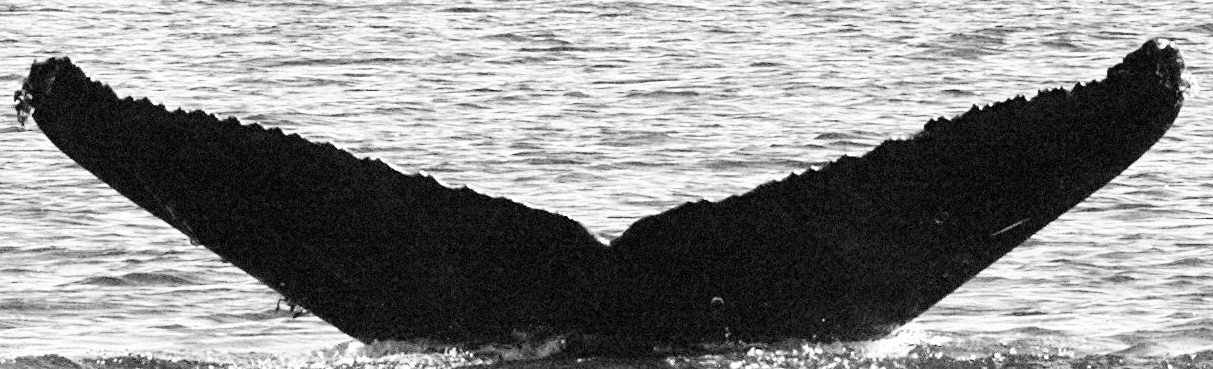
\includegraphics[width=1.0\textwidth]{../images/unclear_texture.jpg}
\caption{\textbf{Uniform Internal Texture}. This image of a humpback fluke shows no clear internal texture, but a distinctive trailing edge.}
\label{fig:unclear_texture}
\end{figure*}

While trailing edge matching has seen limited use in humpback whale identification, it is a much more common technique in sperm whale (P.\ macrocephalus) identification \cite{huele2000finding}, \cite{beekmans2005comparison} \cite{whitehead1990computer}, with varying levels of manual effort.
%We detail these methods below as the fluke trailing edge matching paradigm is similar across species.
In Whitehead's work \cite{whitehead1990computer}, points of interest on the trailing edge are entered and catalogued manually along with their positions.
In order to match these trailing edges, all of the points are compared against points on annotated trailing edges in the database, using a distance threshold to ensure locality.
This is a manual method, requiring extensive annotation for matching.

The method proposed by Huele et al.\ \cite{huele2000finding} uses a semi-automatic extraction of sperm whale trailing edge, and then applies wavelet transformations which are cross-correlated to determine a similarity measurement.

An investigation of the above methods for sperm whale identification is carried out in \cite{beekmans2005comparison}, showing that combining these two methods yields an 80\% top-1 accuracy (meaning that the correct identity is ranked at the top of the potential matches 82\% of the time) on a slightly smaller dataset than ours.
However on their own each method only achieves about 65\% top-1 accuracy.

\begin{figure*}[t]%
\centering
\subfloat[][]{
	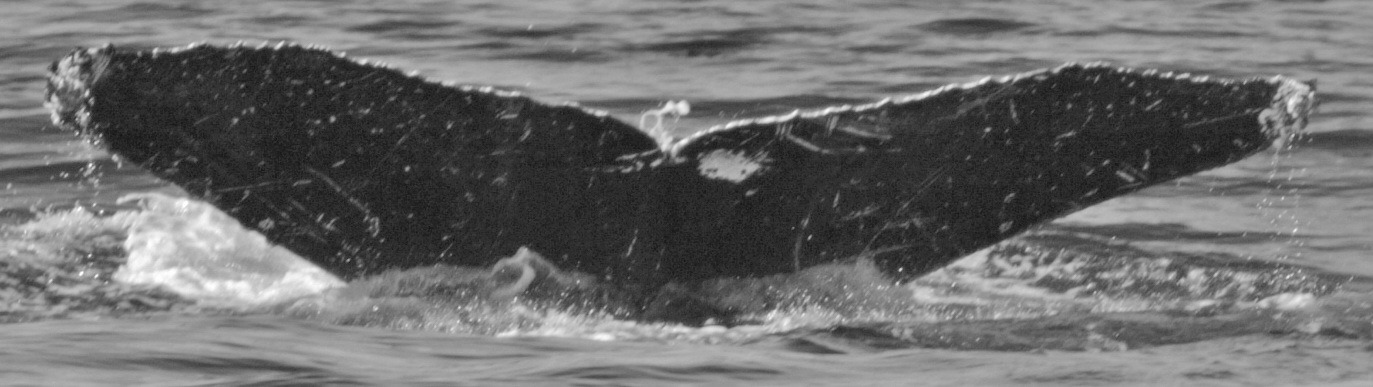
\includegraphics[width=1.0\textwidth]{../images/unclear_te_q.jpg}
}
\newline
\subfloat[][]{
	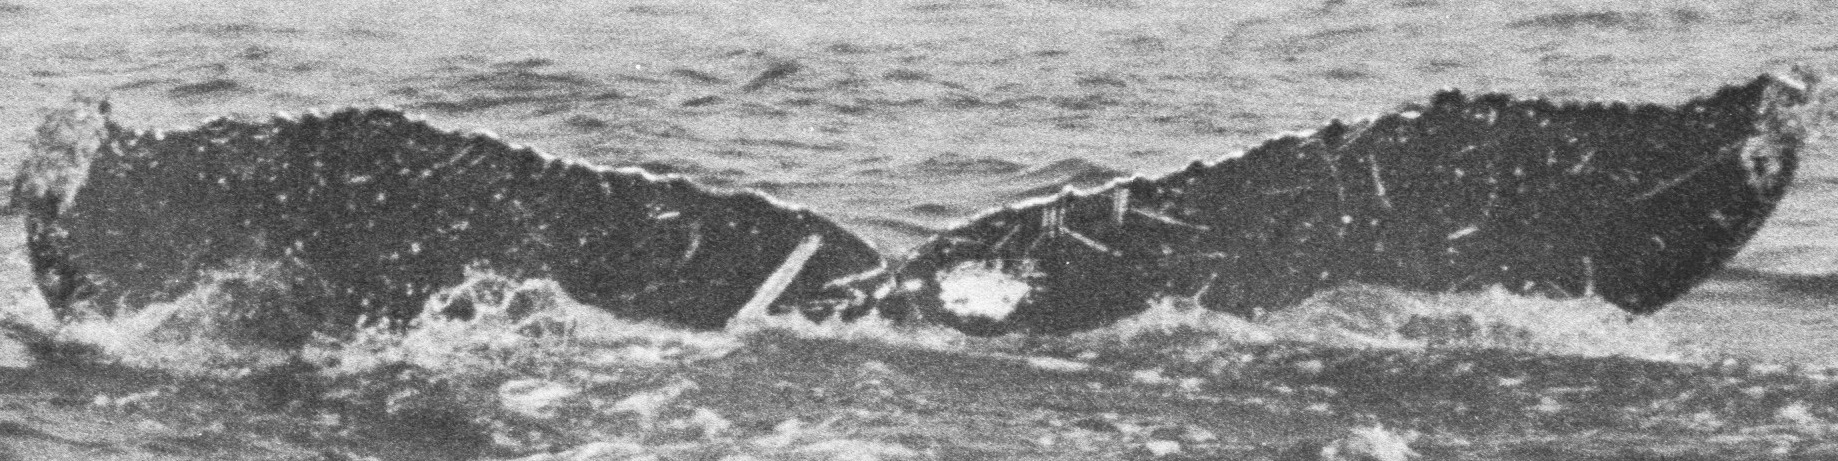
\includegraphics[width=1.0\textwidth]{../images/unclear_te_gt.jpg}
}
\caption{\textbf{Change in Trailing Edge}. The above images show that out of plane rotations of the fluke can obscure it or otherwise make it hard to match. These images are both of the same individual, however in the top image the fluke is rotated slightly towards the camera.}
\label{fig:unclear_te}
\end{figure*}

\subsection{Based on general Fluke appearance}


The primary method for computer-assisted photo-identification of humpback whale flukes is to use the internal fluke pattern, as seen in the work of Mizroch et al.\ \cite{mizroch1990computer} and Flukematcher \cite{kniest2010fluke}. 

In \cite{mizroch1990computer}, information about the fluke is manually catalogued and used to match individual whales. 
The fields that are catalogued contain information primarily about the overall coloration patterns of the fluke, as well as the shape of the central notch. 
The matching algorithm generates potential fluke matches by looking at how similar the annotated patterns are.
This requires significant manual effort to identify individuals.

In Flukematcher \cite{kniest2010fluke}, control points are manually annotated which allow the program to automatically find pigmentation patterns in the fluke and align accordingly.
Optionally distinctive fluke patterns can also be selected by the user.
A variety of heuristic features are then extracted, which are matched using a variety of similarity measures.
This method has acheived a 82\% top-1 accuracy  on a smaller dataset than ours.
However, it requires significant manual effort on the order of five minutes per fluke photograph.

\section{Method Outline}

%TODO: What algorithm is based on

In this thesis, we develop and present an efficient fully-automated\footnote{With the caveat that manual annotation is needed to train parts of the algorithm} algorithm that identifies humpback flukes based on their trailing edges.
For each fluke, the algorithm first determines the left and right tip points of the fluke (as well as the bottom of the central notch). 
The trailing edge contour is then extracted between the left and right tip points, and for each point on this contour curvature is measured at multiple scales.
Once these curvatures are extracted for each fluke photograph, the algorithm identifies a query curvature by computing a distance from it to each database curvature with dynamic time warping.
The query fluke is then identified with the identity of the database fluke with the lowest distance.

%\begin{itemize}
%	\item Find the left and right tips of the fluke
%	\item Extract the trailing edge contour betweeen these points
%	\item Compute the curvature of the trailing edge contour at multiple scales
%	\item Determine a ranking of possible identities using a distance computed by dynamic time warping 
%\end{itemize}

%TODO: Reference / put in (up to chuck?) pictures showing these steps

We also show we can greatly improve the accuracy of this method by combining it with matches found by Hotspotter, a generalized pattern based identification method that is a powerful matching algorithm for several species \cite{crall_hotspotter_2013}.
Hotspotter identifies multiple salient SIFT keypoints in an image that are then spatially verified and matched with other keypoints in the database to produce a ranking over possible identities. %TODO: What does Chuck want me to say about Hotspotter?
Despite the general nature of this method, we find that it does not identify keypoints on the trailing edge and thus struggles with flukes that have no significant internal texture. 
This work is the first to our knowledge that details Hotspotters efficacy when applied to humpback whale flukes, and the results are presented in Chapter 4.
%It should be noted that we used a segmenting convolutional network to aid Hotspotter's predictions, although this is not detailed in this work.

\section{The Dataset}

The main dataset that is used and evaluated in this work is a subset of the dataset collected by the SPLASH project \cite{calambokidis2008splash}. 
It consists of about 1400 identified photographs spread over about 860 identified individuals.
Of these, only 433 individuals have more than one image associated with them, giving 942 images that can be used in a one-to-one comparison.
We refer to this dataset as the Flukebook dataset, which is the team from which it originates. % TODO: make sure this makes sense.

Additionally, an external dataset of unidentified (but annotated) humpback flukes is used for training individual components of the method.

\section{Thesis Outline}

% Main body background in chapter 2
% Primary method in chapter 3, as well as a brief description of some of the alternative methods that were tried
% Reesults presented in chapter 4
% Discussion and future work presented in chapter 5

The rest of this thesis starts by giving a background on the algorithms that our method is based on in Chapter \ref{sec:background}.
Afterwards, the main method is detailed in Chapter \ref{sec:methods}, along with a description of some alternate methods that failed to work as well.
Chapter \ref{sec:results} goes into the results, failure cases, and success cases of the primary algorithm as well as various parameter changes and how they affect the results.
We also describe the effectiveness of this identification method in combination with Hotspotter.
This thesis concludes with a discussion on the failings of the primary method, as well as ways to improve it and generalize it to extracting and matching edge characteristics in other animals.

%TODO: this gud?

The primary contributions of this work are the individual components of the main method for extracting trailing edges and fluke keypoints, as well as the combination of all the components into a coherent identification pipeline.
We also contribute an evaluation of dynamic time warping on curvature measures as a method for matching humpback flukes, as well as an evaluation of Hotspotter for this task.



% Contributions
% A convolutional network and loss for extracting fluke keypoints
% A simple trailing edge extractor for humpback flukes
% A convolutional network for predicting where the trailing edge is
% Curvature extraction and matching algorithm



%\section{Method Overview}

%The method for trailing edge identification put forth in this thesis is very nearly fully automated, requiring no human annotation when used (although manual annotation is necessary for training the machine learning models used).
%On its own, it achieves decent results on a (relatively) large dataset, comparable with the fully automated method used in \cite{hughes2015automated}. 
%Ultimately we find that this method is best used in combination with an automated pattern matching method (e.g. Hotspotter) to provide high accuracy matches.
%We also explore alternative methods based on more recent advances in deep learning for identification, however it appears that the dataset is too small to properly train these methods.


%%% Local Variables: 
%%% mode: latex
%%% TeX-master: t
%%% End: 
 % chapter 1
%%%%%%%%%%%%%%%%%%%%%%%%%%%%%%%%%%%%%%%%%%%%%%%%%%%%%%%%%%%%%%%%%%% 
%                                                                 %
%                            CHAPTER TWO                          %
%                                                                 %
%%%%%%%%%%%%%%%%%%%%%%%%%%%%%%%%%%%%%%%%%%%%%%%%%%%%%%%%%%%%%%%%%%% 
 
\chapter{Background} \label{sec:background}

In this chapter, we provide a series of sections detailing background information on the algorithms on top of which our trailing identifier was developed.
We describe some of the applications and variants of deep convolutional networks on top of which we build our fluke keypoint and trailing edge extractors.
We briefly introduce the concept of seam carving as it relates to our trailing edge extraction algorithm, and provide a small overview of contour curvature measures.
Additionally, we describe briefly the concept of dynamic time warping for sequence matching.

\section{Convolutional Networks}

In recent years, convolutional neural networks have provided state of the art results in several challenging computer vision tasks, including general image classification \cite{krizhevsky2012imagenet}, \cite{szegedy2015going}, image segmentation \cite{long2015fully}, \cite{chen2014semantic} and individual identification (specifically for human faces) \cite{fan2014learning}, \cite{schroff2015facenet}.

The essential idea of a convolutional network is that it we can use the gradient of an error signal to learn hierarchies of convolution kernels separated by nonlinear activation functions.
These networks are considered to be a form of neural network where the convolutions provide a meaningful prior when applied to data with spatial relationships (e.g.\ image data).
Convolutional were introduced nearly 40 years ago by Fukushima in \cite{fukushima1979neural}.
The current incarnation of these networks can be traced back to the seminal work of LeCun et al.\ \cite{lecun1998gradient}.
Modern convolutional networks follow a common framework of using Rectified Linear Units (ReLUs) as activation functions, and Dropout \cite{hinton2012improving} layers after fully connected layers for regularization. % TODO: Clear up w/chuck hoow much detail is needed for this 
Additionally, the convolutional kernels used are commonly small square kernels with ``same'' padding alternated with $2\times$ downsampling layers (specifically max pooling layers) \cite{simonyan2014very}, \cite{sermanet2013overfeat}, \cite{krizhevsky2012imagenet}. % TODO more citations for this

The convolutional networks used in this thesis follow the above framework, and also use batch normalization \cite{ioffe2015batch} at every layer.
We also use orthogonal initialization \cite{saxe2013exact} at all layers to help ensure gradient flow.

\subsection{Facial Keypoint Prediction}

Facial keypoints are essentially coordinates on an image of a (human) face that detail the locations of nose, eyes, mouth, etc.
They are commonly used in facial identification pipelines \cite{taigman2014deepface}, as well as in motion capture \cite{akagi2013facial} and expression recognition \cite{berretti20113d}.
There has been recent work in using convolutional networks for facial keypoint prediction \cite{sun2013deep}, \cite{nouri2014using}. 
The essential idea behind these networks is that they predict points (rather than classifications) in the form of $(x, y)$ coordinates, and are trained with a regression loss function.
In this work, we adjust these methods to predict fluke keypoints marking the left and right tips of the trailing edge using essentially the same paradigm as the above works.

\subsection{Fully Convolutional Networks}

Classically, convolutional networks reduce an image to a single (spatially invariant) vector, which is then used for classification (or embedding, regression, etc.)
To do this, these networks usually have fully connected (or dense) layers towards the end.
This ensures that the receptive field of the network covers the entire image, which is practical for many applications where a scalar or fixed size prediction is required. 
However, when dealing with arbitrarily sized images, it is useful to use networks that are ``fully convolutional'', in which case the entire network consists of convolution kernels. 
Convolutional networks that reduce to dense layers can be cast as fully convolutional networks by replacing the dense layers with $1\times1$ kernels, using the dense units as channels.
This technique is especially applicable in segmentation tasks \cite{ning2005toward}, as this process allows for (downsampled) predictions spatially distributed throughout the image. % TODO More citations eventually
By then upsampling and combining different stages of prediction, the authors in \cite{long2015fully} produce high quality image segmentations, a technique that we replicate for classifying pixels as being part of the trailing edge.
In this work, fully convolutional networks are used for predicting the 'trailing edginess' of an image, which allows us to refine the trailing edge contour extraction. 

%\subsection{Embedding Networks}

%One major difference between the way that individual identification is done with convolutional networks and the standard classification architecture technique is the way that the error to the network is represented.
%When convolutional networks are used for classification tasks, the standard approach is to use a softmax output layer and learn with the cross-entropy loss.
%While an individual identification task could be expressed as a classification task, it becomes a major issue when a new individual is added to the dataset (which for our task should be very common).
%A better notion for the loss function is to make it teach the network to 'embed' images into some $d$-dimensional vector (usually constrained to be unit norm).
%This is generally done by using a loss function that encourages grouping images of the same individual closer than those of different individuals.
%The most common approach to this is to use the contrastive loss \cite{fan2014learning} \cite{chopra2005learning}, although more recently the triplet loss has risen in popularity \cite{schroff2015facenet} \cite{parkhi2015deep}.

\section{Seam Carving}

Seam carving is a technique that tries to resize images without warping or distorting the objects shown in the image \cite{Avidan:2007:SCC:1276377.1276390}.
This technique uses a dynamic programming algorithm to find minimal salience paths through an image, where salience is often defined as the gradient.
The motivation for this is that these minimal saliency paths are not important to the image, so they can be removed to reduce its size.
While this method is not directly used in this work, the underlying algorithm for trailing edge extraction is essentially a single iteration of the seam carving algorithm, using gradient information.

\section{Curvature Measures}

Contour curvature measures are commonly used to characterize the overall shape of an contour. 
A lot of work has been done on using curvature information for detection \cite{monroy2011beyond}, classification \cite{fischer2014image} \cite{kumar2012leafsnap}. % Chuck note: Explain more? Figure out what that means
This curvature information can be broadly broken down into either integral or differential curvature, and is usually computed at multiple scales.

Differential curvature can generally be seen as measuring the angle of the tangent normal of the gradient at each point in an image \cite{fischer2014image}.
For our purposes, we can then take only those points that lie on the contour and use their curvature.
While doing this directly can be fast to compute, it tends to be noise sensitive and we found that integral curvature (below) works better for our purposes.

Integral curvature works (conceptually) by sliding a circle of some radius $r$ along the contour \cite{pottmann2007integral}, and measuring how much of the circle is 'inside' the contour.
This measurement is usually taken at multiple scales, and has the appealing property of being invariant to rotation and translation (of the entire contour).
In this work, we approximate the circular curvature with a square of size $r$, which appears to perform just as well but can be computed much faster.

\section{Dynamic Time Warping}

In deciding a sequence comparator, one criterion that is often important is ensuring that small shifts in the sequence do not balloon into large differences.
Dynamic Time Warping (DTW) is a sequence comparison method that, roughly, finds the optimal matching between all sets of points in the two given sequences that minimizes the overall distance (for some defined distance function) between the matched points, while keeping the locality of the points intact \cite{sakoe1978dynamic}.
This allows for shifts and some warps in the two sequences to be compensated for, and results in a nonlinear mapping of one sequence onto another.
The algorithmic complexity of dynamic time warping can be limiting in large datasets, as it is quadratic in both space and time -- making a one-to-one comparison a bit daunting.

There are several variants on DTW that give faster speeds \cite{salvador2007fastdtw} \cite{lemire2009faster}, however we only use the Sakoe-Chiba bound \cite{sakoe1978dynamic}, which both constrains the neighborhood in which points can be matched and gives a complexity of $O(nT)$, where $T$ is a user set parameter constraining the neighborhood.

Sequences of curvature measures have been used with DTW for signature verification \cite{munich1999continuous}, however this combination has not been used for matching trailing edges to our knowledge.

%%% Local Variables: 
%%% mode: latex
%%% TeX-master: t
%%% End: 
  % chapter 2
%%%%%%%%%%%%%%%%%%%%%%%%%%%%%%%%%%%%%%%%%%%%%%%%%%%%%%%%%%%%%%%%%%% 
%                                                                 %
%                            CHAPTER THREE                          %
%                                                                 %
%%%%%%%%%%%%%%%%%%%%%%%%%%%%%%%%%%%%%%%%%%%%%%%%%%%%%%%%%%%%%%%%%%% 
  
\chapter{Methods} \label{sec:methods}

In this chapter, we detail the finalized algorithm pipeline, as well as some alternative approaches that we found to have limited successs.

\section{Trailing Edge Extraction}

Extracting good, high quality trailing edges images is one of the primary challenges when matching Humpback whales by their trailing edge.
In this section, we describe the steps that go into automating the extraction of high quality trailing edges, while trying to minimize human intervention.

One major assumption we make when extracting these trailing edges is that the humpback whale fluke is aligned such that its major axis is horizontal.
Additionally, we generally assume that all parts of the fluke are present, however theoretically it would be possible to match a partial fluke -- although unlikely.

While these assumptions do not make for an incredibly robust system, the nature of the problem (and the dataset that we had at hand) makes these assumptions reasonable.
It would also be possible to add a detection step beforehand to ensure this assumption, however we do not explore this in this work.

\subsection{Fluke keypoint prediction}


\begin{figure*}[t]%
\centering
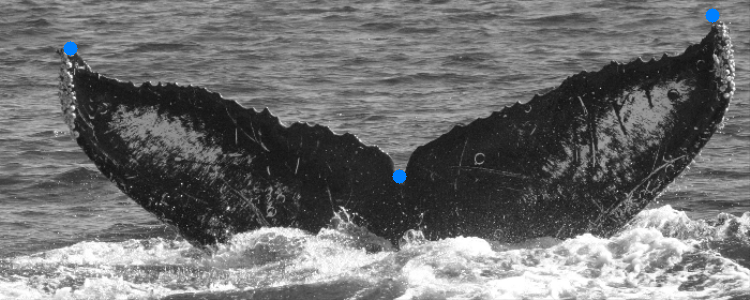
\includegraphics[width=1.0\textwidth]{../images/aid88_kpoverlay.png}
\caption[]{\textbf{Example Keypoint Prediction}. Example image showing the left tip, bottom of the notch, and right tip located by the keypoint extractor convolutional network.}
\label{fig:example_kp}
\end{figure*}


One major issue with automating the above trailing edge extraction algorithm is that it requires manual annotation in the selection of the starting and ending points (i.e., the fluke keypoints), as well as any control points (specifically the bottom of the notch).
To work around this, we propose a convolutional network that predicts these tip points as part of the identification pipeline.

When extracting trailing edges, one of the first steps we take is to identify the starting and ending points of the trailing edge, as well as the bottom of the central notch.
To do this, we train a convolutional network to predict these three points.

The convolutional network does not need full-sized images, so the first step of the keypoint extraction pipeline is to resize the image to $256 \times 256$ pixels.
This size choice is somewhat arbitrary, but we find that it provides the best performance without using an unnecessary amount of memory.
The network then predicts the points as values between $0$ and $1$, for both the width and height of the image. 
These predictions are then then rescaled back up to the original image size.
An example prediction is shown in Figure \ref{fig:example_kp}.
%The evaluated network architectures are detailed in Table 3.1. % TODO put this in

\subsubsection{Network Design}

The overall design of the network follows the pattern of alternating small ($3 \times 3$) convolutional filters with $2 \times 2$ max pooling layers, at each step doubling the number of channels (starting with $8$ channels).
This is somewhat similar to VGG-16, although with half the trainable layers.
After a $32\times$ downsample has been achieved, we attach a decision layer which consists of a dense layer followed by three separate dense layers with separate predictions layers after (one for each point being predicted).
While this is not a common approach in keypoint prediction, we found that it gave better performance than having the points predicted as a single vector.

We theorize that this may be because shared units between each of the three predictions leads to stronger correlations between them, reducing overall prediction flexibility.

\subsubsection{Training Details}

Generating the training data for this is straightforward given a set of annotations with the associated points to learn.
The dataset that we created for this purpose contains approximately $2100$ training images, $700$ validation images, and $900$ test images.

First, each image is resized to a fixed width while maintaining the aspect ratio.
This is done to somewhat normalize the relative scale of objects in each image on the assumption that they are constrained to contain the fluke.
Each image is rescaled to the network size, and then the corresponding targets are rescaled to the range $[0-1]$.
The size of the original image is recorded as well.
While it would be possible to treat this as a simple multi-variate regression and use RMSE loss, we achieved better results by averaging the Euclidean distance between the predicted points and true points.
We also include a scalar scaling factor $\alpha$, which scales each point by a proportion of the original image size.
Thus, we have the scaled Euclidean loss $SE$

\begin{equation} \label{eqn:se_loss}
SE(\vec{t}, \vec{p}, \vec{s}, \alpha) = \lVert (\alpha * \vec{s}) \odot (\vec{t} - \vec{p}) \rVert
\end{equation}
Where
\begin{itemize}
    \item $\vec{t}$ and $\vec{p}$ are the $(x, y)$ ground truth and predicted values respectively
    \item $\vec{s}$ is the original image width and height
\end{itemize}

The networks are trained for 1000 epochs with $\alpha$ set to \num{2e-2} using the Adam \cite{kingma2014adam} optimizer (with recommended settings) and $l2$ regularization on the trainable parameters with a decay of \num{1e-4}.
All of these hyper parameters were tuned using the validation set, although the possible parameter space was not fully explored due to time constraints.

\subsubsection{Evaluation} % TODO: Maybe this should be moved to the results section?

%TODO Put in a bunch of figures and talk about this
% Problem is recreating all these experiments / networks for evaluation :/
% Might take a while...

On average, the best network achieved a 10 pixel distance error on the validation and testing sets (in the original image scale).
While this may seem like a lot, the trailing edge extraction (and subsequent matching accuracy) was not severely affected when only using the start and end point predictions.

%Additionally, as can be seen in Figure 3.2, 
We find that, for the vast majority of images, the network achieves a low pixel distance error, while there are a few that have a much higher error.
Qualitative inspection of these images shows that they are either of flukes which are not the singular or major object in the image, or horizontally oriented of flukes that are not horizontally rotated.
An example of this is shown in Figure \ref{fig:example_kp}.

%  TODO: Figure showing this

\begin{figure*}[t]%
\centering
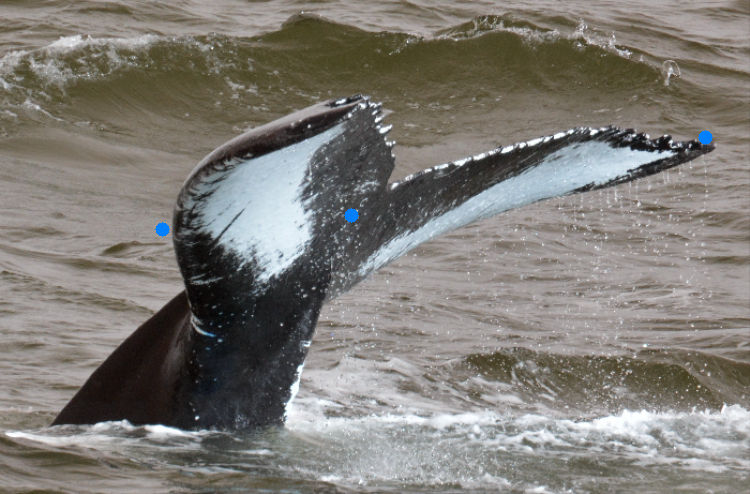
\includegraphics[width=1.0\textwidth]{../images/aid1323_kpoverlay.png}
\caption[]{\textbf{Example Keypoint Failure}. Example image showing a keypoint extraction failure case from its testing set. Note the difference in pose of the fluke from the success case shown in Figure \ref{fig:example_kp}}
\label{fig:example_kp_failure}
\end{figure*}



We attempted to use a spatial transformer network \cite{jaderberg2015spatial} to try and handle these cases, but we were unable to get it to perform as well as the standard convolutional network, nor produce sensible transformations.
Since these failure cases represent a small amount of the dataset

\subsection{Basic Trailing Edge Extraction Algorithm}

% TODO: Picture of I_y

The base algorithm that is used for extracting the trailing edge uses the vertical gradient information of the image (denoted as $I_y$).
We extract $I_y$ using a vertically oriented $5 \times 5$ Sobel kernel \cite{Sobel1968}.  

We then normalize $I_y$ with min-max scaling, giving $N_y$ as

\begin{equation} \label{eqn:norm01}
N_{y} = \frac{I_y - \min(I_y)}{\max(I_y) - \min(I_y)}
\end{equation}

With $N_y$, we then need a starting point and ending point for the algorithm, denoted $s$ and $e$ respectively, with their $x$ and $y$ coordinates being denoted with subscripts. 

For our purposes, we use the left and right tips of the fluke as our start and end points respectively.
Additionally, we experiment with using the bottom of the notch to aid the trailing edge extractor.
We explain how these points are determined in the next section.

Given a point $p$, we then set its corresponding column in $N_y$ to $\infty$, and set the point itself set to $0$. 

\begin{align} \label{eqn:te_setup}
N_y(p_x,\cdot) = \infty \\
N_y(p_x,p_y) = 0
\end{align}

This forces the path to ``go through'' these points. 
We do this for the start (i.e.\ left tip) and end points, as well as the bottom of the notch. 

The minimal path is then found by scanning the columns of $N_y$ from left to right, starting and ending at $s$ and $e$ respectively. 
For each pixel in a column we set its cost with the following update rule:

\begin{equation} \label{eqn:te_update}
C(x,y) = 
\begin{cases}
	0 & x < 0 \\
	\infty & y < 0 \text{ or } y > h \\
	\min_{y - n \leq y_c \leq y + n}(C(x-1, y_c) + N_y(x,y)) & \text{else} \\
\end{cases}
\end{equation}

Where $n$ is a neighborhood constraint and $h$ is the height of $N_y$.  
We default $n$ to $1$, meaning that each pixel considers $3$ 'neighbors' in the previous column.

As $C$ is filled out, we also keep a backtrace matrix $B$, which keeps track of the index of the minimal candidate chosen in equation \ref{eqn:te_update}.
Once the end column is reached, we work backwards from $e$ to construct the path, adding the coordinate corresponding to $B(x,y)$ at each step.

% Maybe: Put in actual algorithm pseudocode
% TODO: Put in pictures of extracted fluke, cost matrix?

We can also extend this algorithm by adding extra 'control points' which the path is forced through, using the same methodology as forcing the path through the start and end points.
Commonly, we use the bottom of the notch as a control point, although this affects accuracy negatively if it too far from the trailing edge.

While this algorithm has no understanding of humpback whale flukes, a lot of images that are constrained around the fluke with oceanic backgrounds (which is a large majority of the dataset at hand) provide high quality trailing edges when put through this algorithm.
However this is not a robust algorithm for finding trailing edges, something that we will fix later on.

% TODO: Put in figure showing bad trailing edge from raw next to good one

\subsection{Trailing Edge Scoring}

As mentioned in the beginning of this section, using only the gradient information for extracting the trailing edge works in a lot of cases, but is not a robust method.

If we had a score of each pixel's ``trailing edginess'' in an image, the trailing edge extractor could make use of this information to make better choices in trailing edge extraction.
To do this, we need a prediction of whether or not each pixel belongs to the trailing edge of a fluke, a task that is best suited to a fully convolutional network.
In these networks, all convolutions (aside from max pooling layers) are ``same'' convolutions, which have square, odd filters (usually $3 \times 3$) and 1-padding. % TODO: Maybe find a citation describing these?
These ``same'' convolutions produce a spatial output shape that is the same as the input shape, obviating the need for any interpolation.

The four major variants on trailing edge scoring networks that we evaluated are detailed below.
All of these networks function on the same paradigm of taking an arbitrarily sized image and producing an image of the same size but with a class score for each pixel.

The dataset was sourced from trailing edges extracted using the basic method detailed above, however with manual adjustments to fix many of the more common issues we encountered with this algorithm.

To generate the training set, we extract a $128 \times 128$ patch at $128$ pixel intervals along the trailing edge (giving a positive patch), and a corresponding patch (with no trailing edge pixels) randomly sampled from the left over space above and below the trailing edge (giving a negative patch).
These patches are then randomly split into training, testing, and validation sets each with $3700$, $1200$, and $1600$ patches respectively.

\subsubsection{Trailing Edge Scoring Architectures}

There are several network architectures that were tried, however here we will report only the major variants.
One major consideration that has to be made when selecting a fully convolutional network architecture is its receptive field.
If the receptive field is too small, it may not have enough information to accurately determine if a given pixel is part of the trailing edge.
However, in order to increase the receptive field without massively increasing the depth of a network, we must downsample, which makes the output less fine-grained.

\paragraph{Simple}
This network is simply a stack of $6$ "same" convolutional layers (of decreasing spatial extent), with no downsampling regions.
This has a small receptive field, but can produce detailed predictions.
Due to the small receptive field however, at convergence it gives low precision predictions, and seems to (in many cases) produce a lot of the same mistakes that normal gradient based trailing edges do.

\paragraph{Upsample}
To deal with the small receptive fields, convolutional networks typically downsample at various stages. 
This downsampling usually takes the form of max pooling (instead of e.g. convolutional kernels with a stride greater than one).
The upsample architecture is analogous to the FCN-32s architecture in \cite{long2015fully}, although we do not go down to a 1x1 spatial extent before upsampling.
This produces blocky and nearly unusable trailing edge scores, however they tend to be more connected than the disparate (but fine-grained) predictions made by the simple network.


\paragraph{Jet}
Following the deep-jet architecture from \cite{long2015fully}, we combine softmax predictions from various stages throughout the network with predictions from "farther down" the network, cascading until we hit predictions from the last convolutional layer before any downsampling.
This gives more fine-grained predictions than the upsample network while giving somewhat better predictions than the simple network.


\paragraph{Residual}
While the receptive field of the Simple network is small, it can produce very fine trailing edges, which we found to be necessary for good trailing edge extraction.
However with such a small receptive field it can be more prone to making mistakes.
It is possible to create a very deep network of 'same' convolutions, however training very deep networks like this can run into problems very quickly.
Recently, there has been work on making very deep networks feasible by adding residual connections\cite{he2015deep}, showing that these very deep networks can achieve high accuracy in a challenging benchmark.
We replicate this architecture by stacking $64$ $3\times3$ 'same' convolution kernels, and adding a residual connection every other layer.
This performs better than the Simple network, however we do not see a marked improvement in trailing edge matching as a result.

% TODO: Include images showing extracted trailing edge scores for all of these networks

\subsubsection{Using the trailing edge scores}

Once we have 'trailing edginess' score for each pixel, we need to combine this information with the gradient in a way that causes the trailing edge extraction algorithm to follow those pixels that the scoring map marks as trailing edge.
More formally, the trailing edge scoring map gives us an image $T_p \in [0-1]^{w \times h}$ (where $w$ and $h$ are the width and height of the image) which denotes the network's predicted probability of each pixel being part of the trailing edge.
The most simple and obvious way to combine this information with $N_y$ from before is to combine them with a mixing parameter $\beta$.

\begin{equation}
S_{te} = (1 - \beta)*N_y + \beta*(1 - T_p)
\end{equation}

We use $1 - T_p$ in this case because we are minimizing the path through $S_{te}$.
Once done, the trailing edge extraction algorithm procedes as described in the previous section.

For most of the evaluation process, we simply set $\beta = 0.5$.

Another variant on combining $T_p$ and $N_y$ that we tried was to dilate the trailing edge predictions and then forbid the trailing edge from going outside of those predictions.
However one of the main issues with this is that if there are any breaks in the prediction (which can happen even with the Upsample architecture), the trailing edge cannot be extracted, leading to broken trailing edges.

\subsubsection{Training Details}

All networks were trained for 100 epochs (or until convergence) with a batch size of $32$, with $l2$ regularization using a decay of \num{1e-4}.
We used the Adam optimizer\cite{kingma2014adam} (with the recommended settings) for calculating weight updates.

One detail that turned out to be important is the class imbalance.
The trailing edge pixels (necessarily) make up a small percentage of the total image, meaning that these networks could get a fairly high accuracy (and thus low loss) simply by predicting only background pixels.
In order to prevent this, we only sample a negative patch once for every positive patch (as detailed above), and additionally we weight the loss for the trailing edge pixels $10\times$ higher than the loss for the background pixels.

Due to the nature of the training data, we were concerned that the networks would simply learn to replicate the function that generated the trailing edges, despite human corrections.
In order to mitigate this issue, we included some non-spatial data augmentation, namely random Gaussian blur and randomly inverting the pixel intensities.
Unfortunately this had limited success.

% TODO: Show failures

All of these hyper parameters were tuned using the validation set, although the possible parameter space was not fully explored due to time constraints.

\subsubsection{Evaluation}

Due to the overwhelming class imbalance, the model accuracy is rather meaningless (e.g.\ the accuracy of an all-background prediction is $99\%$).
Instead, we report the intersection-over-union (IoU) score, which gives a much better idea of model performance.
We also report the precision and recall of the model.

% IOU / PRECISION / RECALL
% TRAIN / TEST / VAL
% SIMPLE / UPSAMPLE / JET / RES


\begin{table*}[!htb]%
	\centering
	\resizebox{\linewidth}{!}
	{
		\begin{tabular} {l || l | l | l || l | l | l || l | l | l |}
		& \multicolumn{3}{c||}{Training} & \multicolumn{3}{c||}{Validation} & \multicolumn{3}{c|}{Testing} \\
		\hline
		Architecture & Pr. & Re. & IoU & Pr. & Re. & IoU & Pr. & Re. & IoU \\
		\hhline{=#===#===#===|}
		Simple & 0.59 & 0.95 & 0.57 & 0.59 & 0.94 & 0.57 & 0.60 & 0.95 & 0.59 \\
		\hline
		Upsample & 0.17 & 0.88 & 0.17 & 0.17 & 0.86 & 0.17 & 0.17 & 0.87 & 0.17 \\
		\hline
		Jet & 0.62 & 0.89 & 0.57 & 0.62 & 0.88 & 0.57 & 0.63 & 0.89 & 0.58 \\
		\hline
		Residual & 0.57 & 0.93 & 0.54 & 0.57 & 0.92 & 0.54 & 0.58 & 0.93 & 0.56 \\
		\hline
		\end{tabular}
	}
	\caption{Table showing the precision, recall, and IoU of each of the evaluated trailing edge scorers on each section of the trailing edge dataset. For the purposes of this analysis, we use the \texttt{argmax} over the classes to determine a positive (i.e. trailing edge) or negative pixel.}
	\label{tab:te_score_full_analysis}
\end{table*}

Initially, we thought that precision would be the most important metric for evaluating networks (which is reflected in the class weighting).
However, we found that even a low precision classifier could give good trailing edges, and that the important measure was how detailed these trailing edges were.

% TODO: Figure showing this

This is likely because small segments of predicted trailing edge would not be chosen by the trailing edge extractor if they are too disconnected from the actual trailing edge.

\section{Trailing Edge Matching}

Given extracted trailing edges, we define a method for doing a one-to-one comparison between a given query and database trailing edge.
%Once these trailing edges are extracted, we can use a few simple methods to compare them in search of a trailing edge that is close to the one we are finding a match for.
The simplest way to do this is to define a (potentially non-metric) distance function between any two trailing edges.
Once this distance function is defined, we can identify an individual by its trailing edge (referred to as the query trailing edge) by looking at the identity of the closest trailing edge in the database.
As a distance function we use dynamic time warping over block curvature measurements, using a weighted Euclidean distance as a local distance function between curvatures.

\subsection{Curvature Measurement}

In order to do this, we must first extract the curvature from the trailing edge.
Given the trailing edge as a sequence of coordinates into the original image, we construct a zero-image $I_0$ of shape similar to the original image.
Each pixel corresponding to and below the trailing edge in $I_0$ is set to $1$.
Because the trailing edge extractor produces only one coordinate per column, we can do this safely, however this algorithm could be easily adapted to this not being the case.
Once this is done, we calculate a summed area table \cite{crow1984summed} $ST$ from $I_0$ as follows.

\begin{equation} \label{eqn:sat}
ST(x,y) = \sum_{i=0}^{i=y}\sum_{j=0}^{j=x} I_0 
\end{equation}

Conceptually, the next step is to slide a square of shape $s \times s$ centered on each point, and measure the percentage of that square that is within the filled in trailing edge.
These values $s$ are the different scales at which we meassure curvature, and are computed as a percentage of the trailing edge length.

To do this, we compute $BC_s(x, y)$ for each $(x, y)$ coordinate in the trailing edge.

\begin{align} \label{eqn:sat_area}
\begin{split}
b(i) &= i - \frac{s}{2}\\
e(i) &= i + \frac{s}{2}\\
BC_s(x,y) &= \frac{(ST(b(x), b(y)) + ST(e(x), e(y))) - (ST(b(x), e(y)) + ST(e(x), b(y)))}{s^2}
\end{split}
\end{align}

The numerator in equation \eqref{eqn:sat_area} gives the total area within the square that is below the trailing edge, which we then normalize by dividing by the square's area.

The set of scales to choose presents a large parameter space, however we have found that the scales $S = [2\%, 4\%, 6\%, 8\%]$ work well for our purposes.
We then treat this curvature measurement as a $|S| \times l$ matrix $BC$, where $l$ is the length of the trailing edge.

\subsection{Sequence Matching}

Given two sequences of curvatures $BC_1$ and $BC_2$ (referred to as query and database curvature respectively) we match them using dynamic time warping as follows.
First, we create a cost matrix $C$ of size $l_1 \times l_2$. 
We initialize this cost matrix by setting the first column and row to $\infty$, and then $C(0,0) = 0$, intuitively forcing the optimal path to match align the beginning of $BC_1$ with $BC_2$.
Then, for each cell $(i,j)$ in the cost matrix starting with $C(1,1)$, we use the following update rule

\begin{align} 
\label{eqn:dtw_dist}
D_{\vec{s_w}}(c_1, c_2) &= \lVert \vec{s_w} \odot (\vec{c_1} - \vec{c_2}) \rVert_2\\
\label{eqn:dtw_update}
C(i,j) &= D_{s_w}(BC_1(i,\cdot),BC_2(j,\cdot)) + min(C(i-1,j), C(i,j-1), C(i-1, j-1))
\end{align}

Where $\vec{s_w}$ is a vector giving the weight for each curvature scale, and $\vec{c}$ is a vector of the curvatures at different scales for a point.

Additionally, we impose the Sakoe-Chiba \cite{sakoe1978dynamic} locality constraint $T$ so that for each element $i$ in $BC_1$, we only consider the range over elements $j$ in $BC_2$ of $j \in [min(i - T, 0), max(i + T, l_2)]$.

We set $T$ as a percentage of $l_1$.
For most of these experiments $T$ is set to $10\%$, which appears to minimize the time taken for each comparison while preserving the overall accuracy of the algorithm.

It's worth noting that while this distance measure is not a metric distance (i.e.\ it doesn't satisfy the triangle inequality), it is a symmetric distance as \eqref{eqn:dtw_dist} is symmetric \cite{muller2007information}.

\section{Alternative Approaches}

In this section, we list and briefly describe alternative approaches that were tried, although they did not prove accurate enough to make it into the final system.

\subsection{Aligning Trailing Edges}

One obvious pre-processing step that would make sense when comparing trailing edges is to make sure that they are aligned in image space.
However, we found that doing so when comparing curvature was often unnecessary (due to the invariances to rotation and translation, scale was taken care of separately), and using the Euclidean distance between points on the aligned trailing edges (i.e.\ in place of curvature for \eqref{eqn:dtw_dist}) did not give good results.

There were two approaches to alignment that we evaluated, although neither achieved top-1 accuracies above $20\%$.

\subsubsection{Keypoint Alignment}

As noted in the section on fluke keypoints, there are three points to predict --- left, notch and right.
Originally the intention for recording (and predicting) all three, as opposed to just left and right, was to have three corresponding points with which to estimate an affine transformation from database image onto query image.
This would be done prior to any computation of trailing edge or curvature.

One major issue with aligning these iamges however is that if a non-affine transformation was required, the trailing edge itself would be warped in such a way that made matching difficult.

\subsubsection{Dynamic Time Warping Alignment}

Taking after the AI-DTW approach laid out in \cite{qiao2006affine}, we ran an iterative alignment process that used the correspondences found by DTW (using either curvature distance or Euclidean distance as criteria).
Essentially this method would find alignments using DTW, and then use these alignments to estimate an affine transformation of the database image onto the query image -- and then repeat until convergence.

However, we found that this process oftentimes wouldn't converge, and when it did the alignments provided were of worse quality than those found by aligning the three fluke keypoints.
Additionally, the extra time taken to carry out this process was impractical.

\subsection{Histogram Matching}

One early curvature comparison method that we evaluated was to use histograms to match instead of a sequence-based method.
This is a common approach for comparing curvatures \cite{kumar2012leafsnap}, however we found that for our purposes even high resolution histograms did not provide enough detail to match the trailing edges properly, although this could potentially be explored further.

\subsection{Embedding via Convolutional Networks}

We also made an attempt at training convolutional networks to directly embed the images of flukes into a $n$ dimensional vector, much like \cite{schroff2015facenet} and \cite{parkhi2015deep}.
However, most of the previous literature on this technique is applied to larger datasets such as LFW\cite{huang2007labeled}, which is significantly larger than the dataset that we had available.
A major factor in this is that these larger datasets often have five to ten images per identity (if not more), whereas most of the identities in our dataset had one or two images associated.

Regardless, we attempted the embedding approach (from raw images), however even a severely overfit convolutional network only achieved half the top-1 accuracy on its training set that the main method is able to achieve.
We tried both triplet loss (a modified version of the one detailed in \cite{schroff2015facenet}) and contrastive loss \cite{hadsell2006dimensionality} to no avail.

We believe that the small amount of images per identity is the main factor for the failure of these methods, and that a larger dataset would be necessary to properly train them.

%%% Local Variables: 
%%% mode: latex
%%% TeX-master: t
%%% End: 
 % chapter 3
%%%%%%%%%%%%%%%%%%%%%%%%%%%%%%%%%%%%%%%%%%%%%%%%%%%%%%%%%%%%%%%%%%% 
%                                                                 %
%                            CHAPTER FOUR                          %
%                                                                 %
%%%%%%%%%%%%%%%%%%%%%%%%%%%%%%%%%%%%%%%%%%%%%%%%%%%%%%%%%%%%%%%%%%% 

% EXPERIMENT COMMANDS
% ibeis -e rank_cdf --db humpbacks_fb -a default:has_any=hasnotch,mingt=2 -t default:proot=BC_DTW,decision=max,crop_dim_size=750,crop_enabled=True,manual_extract=True,use_te_scorer=True,ignore_notch=False,te_net=annot_res,te_score_method=avg,equalize_hist=False,kp_net=256_decoupled,tol=10 --dpath=/home/zach/data/results --save=<etc>.png --clipwhite

\chapter{Results} \label{sec:results}

In this chapter we present the results that our primary method achieves on the Flukebook dataset.
The main results for the optimal method are given briefly, and then we discuss how different variations on the method affect accuracy.
We go on to discuss the performance of our method when used in combination with Hotspotter.

\section{Main method}

The main method we settled on achieves an 80\% top-1 accuracy on the Flukebook dataset --- meaning that for 80\% of the query images, the correct identity is ranked first. 
The figures that we show in this section give the accuracy up to top-5 cumulatively.
In general we find that relative accuracies between configurations do not change significantly as we increase the rank at which we allow a match.
\\\\
The optimal configuration that we used for this method is given below.
\begin{itemize}
\item For every image, we predict keypoints by resizing a copy of the image to $128 \times 128$ and running it through the keypoint predictor.
\item Every image is then cropped between the predicted left and right tips, and resized to the same width ($750$ pixels) while maintaining aspect ratio. 
\item We do not use the bottom of the notch as a control point for trailing edge extraction.
\item We set the number of neighbors used in trailing edge extraction $n$ to $3$.
\item We use the Residual architecture for scoring the trailing edge.
\item The trailing edge score is averaged with the normalized gradient (i.e.\ $\beta = 0.5$).
\item We use $M =$ [2\%, 4\%, 6\%, 8\%] for our curvature scales.
%\item We weight all curvature scales equally
\end{itemize}

\section{Configuration Options}

\subsection{Variability in Matching Score}

\begin{figure*}[t]%
\centering
\includegraphics[width=1\textwidth]{../images/results/score_sep_crop.png}
\caption{\textbf{Score Separability Histogram}. The blue bars in this figure represent true matches, and the red bars represent false matches. The line at $\text{score} = 0.88$ represents the optimal threshold at which to accept a match, although we can see it is not perfect.}
\label{fig:score_sep}
\end{figure*}

We find that a major issue with our method is the lack of strong correlation between the distance between two trailing edges and whether or not they belong to the same individual.
We can see this in Figure \ref{fig:score_sep}, which shows that the scores\footnote{The score is computed as $e^{\frac{-\text{distance}}{50}}$ for implementation reasons} between query trailing edges and their corresponding ground-truth trailing edge overlaps heavily with the distance between these queries and unrelated (i.e.\ ground-false) trailing edges.
The result of this is that small changees in the query and database trailing edges can (in some cases) cause the ranking of a ground-truth trailing edge to change significantly.
While this effect is rare given all of the queries, we find that it is the cause of many discrepancies in matching accuracy between different configurations.
With this in mind, we discuss the difference in matching accuracy only when it is a result of significant discrepancies --- meaning that the score between query and ground-truth trailing edge changes by more than $\epsilon = 0.02$ for a significant percentage of the match failures. %TODO: Determine a good value for this

\subsection{Effectiveness of Keypoint Extractor}
\begin{figure*}[t]%
\centering
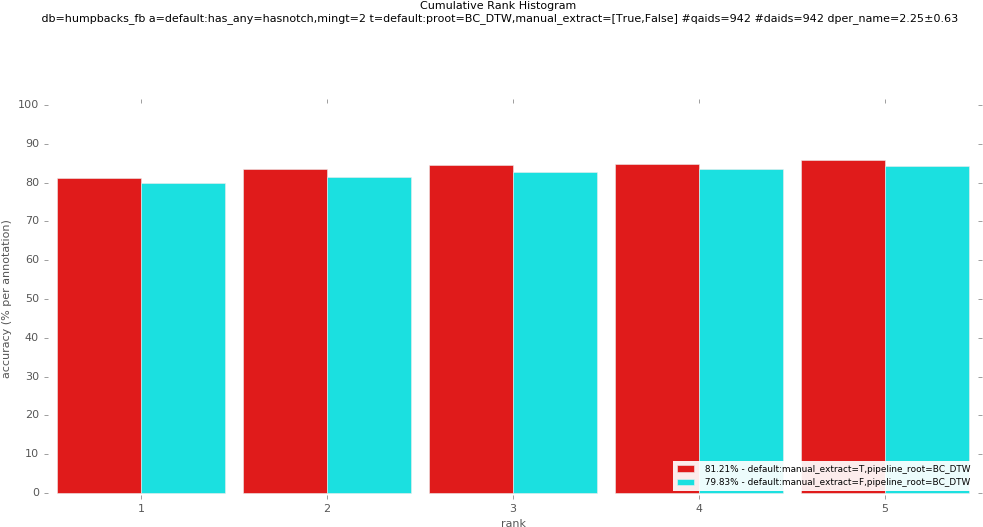
\includegraphics[width=1\textwidth]{../images/results/vary_manual_extract.png}
\caption{\textbf{Varying Manual Extraction}. There is a small difference in matching accuracy between using the manually annotated points (red) provided for this dataset versus the keypoint extractor's predicted points (cyan). The bottom of the notch keypoint is not used in these evaluations.}
\label{fig:vary_manual_extract}
\end{figure*}

In order to test the effectiveness of the trained fluke keypoint predictor, we give a comparison of matching accuracy against manual annotations of fluke keypoints\footnote{Provided with the Flukebook dataset} in Figure \ref{fig:vary_manual_extract}.
While this does not mean that the keypoints predicted are perfect, it does imply that they are ``good enough'' to extract a matchable trailing edge, despite being on average $5$ to $10$ pixels off.
Additionally, we found that only a small percentage of the match failures caused by automatic keypoint prediction were a result of differences in score above $\epsilon$.

%\subsubsection{Keypoint Extractor Image size}

%When predicting keypoints in an image, it is intuitive that the bigger the image the better the prediction can be, but at the expense of requiring more parameters (and thus memory, performance, and model variance) to handle the input.
%We can see in Figure \ref{fig:vary_kp_size}

%The primary difference between the networks that were trained to handle different size inputs is that, in order to ensure that all inputs to the final dense layers have the same spatial size ($2\times2$) across the different networks, an extra convolutional and pooling layer is added.

%\begin{figure*}[t]%
%\centering
%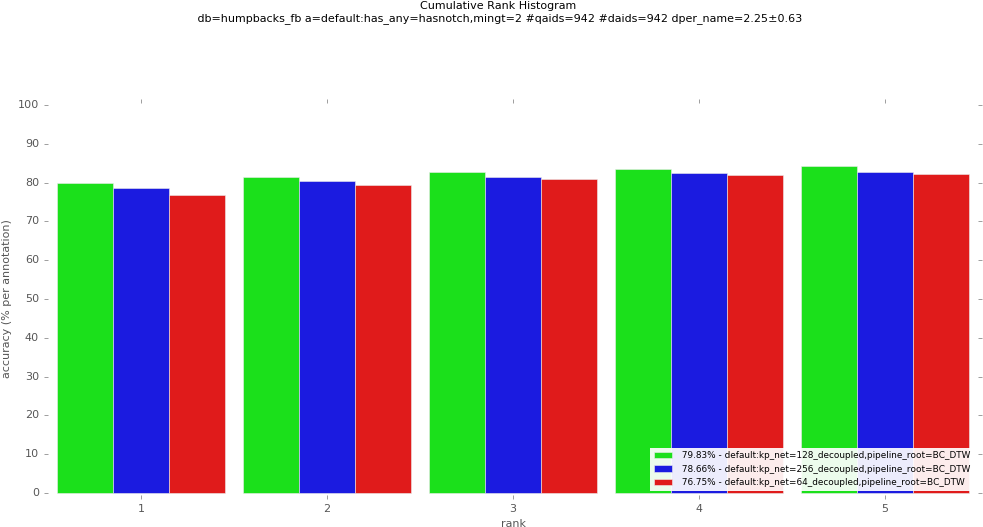
\includegraphics[width=1\textwidth]{../images/results/vary_kp_size.png}
%\caption{\textbf{Varying Keypoint Image Size}. The larger keypoint image size provides a somewhat better accuracy. We did not see an improvement in accuracy beyond an image sizee of $128 \times 128$.}
%\label{fig:vary_kp_size}
%\end{figure*}

%We trained each of these networks on separate splits of data, and due to the inherent stochasticity of the training it is difficult to ascertain whether or not the image size is a cause of performance issues. 

%\subsubsection{STN} % Maybe?

%We also briefly experimented with an Spatial Transformer Network \cite{jaderberg2015spatial}.
%This was largely motivated by the tendency of the keypoint extractor to poorly predict fluke keypoints on flukes that did not ``fill'' the image horizontally.
%Unfortunately, we could not get the STN to converge at a better accuracy than the standard keypoint extractor, even if we held its parameters fixed for a few training epochs.
%Usually, the STN would produce nonsensical transformations of the image.

\subsection{Cropping Width}


With dynamic time warping, we theoretically can match trailing edges of arbitrary lengths --- however the distances can be distorted by large differences in actual trailing edge length.
For this reason we fix the length of the trailing edges.
Since we are only interested in the width of an image (because of the way the trailing edge extraction algorithm works), we can get every trailing edge to have exactly some fixed length $w$ by the following process.

\begin{itemize}
    \item Crop the image horizontally between the left and right columns found by the keypoint extraction process (or manually determined).
    \item Resize the cropped image to some fixed width $w$ while preserving the aspect ratio.% using Lanczos interpolation. % Maybe find citation for this
\end{itemize}

\begin{figure*}[t]%
\centering
%\subfloat[Distribution of Image Widths][]{
%	\includegraphics[width=0.5\textwidth]{../images/results/chip_width_hist_fb.png}
%}
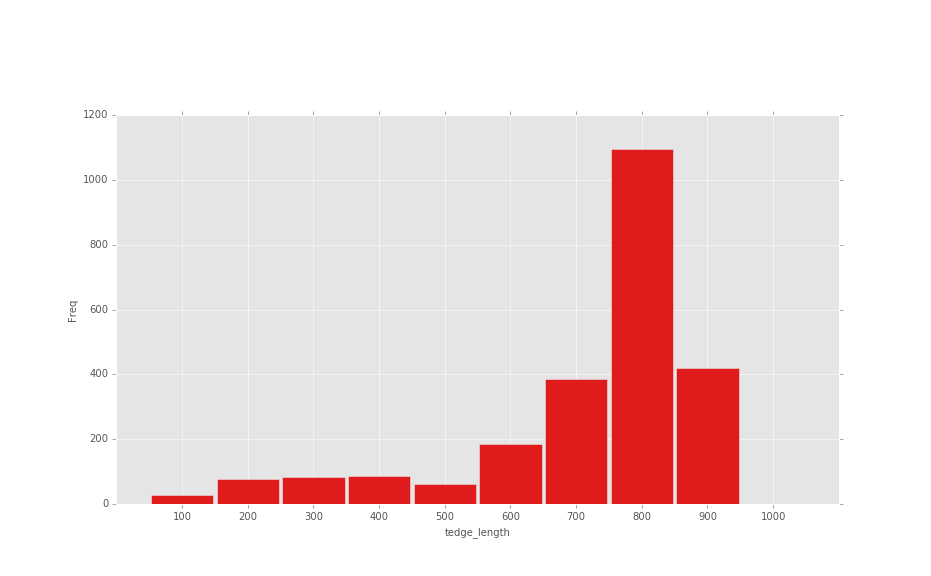
\includegraphics[width=1\textwidth]{../images/results/te_size_hist_fb.png}
\caption{\textbf{Distribution of Unresized Trailing Edge Lengths}. This shows a significant distribution of trailing edges centered around a width of 800 pixels.}
\label{fig:width_te_dist}
\end{figure*}

In this way, we standardize the trailing edge length so that differences in image size do not affect detection accuracy.
One major caveat with this process is of course that using the keypoint extractor's predictions can cause catastrophic failures in this process (e.g.\ if the left and right points are nowhere near a fluke), however in practice we found that this is not an issue.

%We can see in Figure \ref{fig:vary_crop_nocrop} that cropping and resizing is absolutely vital to the performance of our algorithm.

%\begin{figure*}[t]%
%\centering
%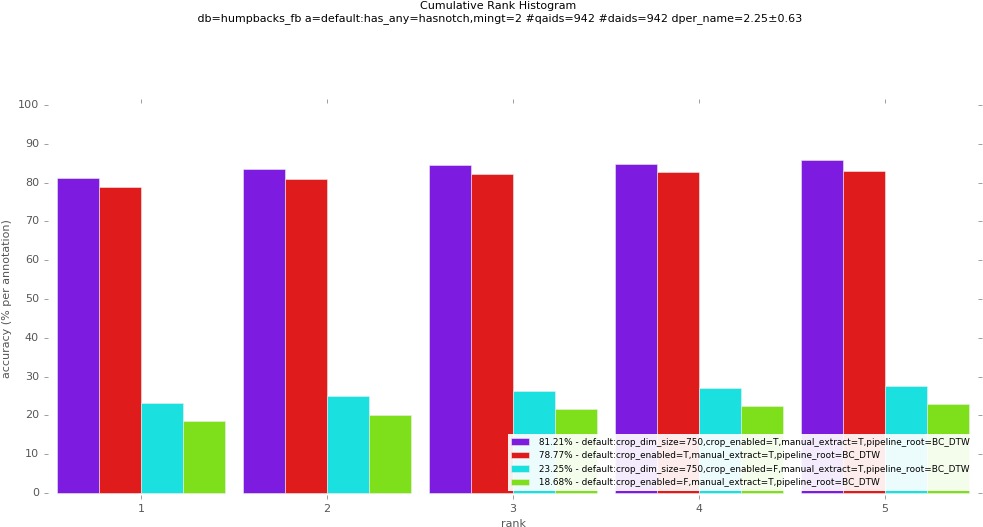
\includegraphics[width=1\textwidth]{../images/results/vary_crop_nocrop.png}
%\caption{\textbf{Varying Crop Strategy}. Cropping images around the trailing edge and then resizing them proves to be very important, not doing so gives a very low accuracy. We can see in Figure \ref{fig:chip_size_hist} that there is a wide distribution of image sizes, which can hamper the effectiveness of DTW.}
%\label{fig:vary_crop_nocrop}
%\end{figure*}

%We also note that we originally tried histogram equalization as part of the preprocessing pipeline, although it produced significantly worse trailing edges (and subsequently matching accuracy).

Ideally, we would choose a $w$ that minimizes the interpolation artifacts that result from making big changes in image size.
Figure \ref{fig:width_te_dist} shows the histogram of post-crop widths (i.e\ trailing edge lengths) from unresized images in the Flukebook dataset, showing a large concentration of mass around 800 pixels. 
Subsequently, Figure \ref{fig:vary_crop_size} shows that $w = 750$ performs well, although $w = 1000$ is on par.
We select the former for efficiency's sake, as smaller trailing edges vastly improves the speed of the matching algorithm.
This provides evidence for the hypothesis that the less the image has to be resized, the better the trailing edge.

\subsection{Trailing Edge Extraction}

One major result that we found was that, when using the averaging method to combine the trailing edge scores with $N_y$, having a robust trailing edge prediction wasn't as important as having a detailed trailing edge.

\begin{figure*}[t]%
\centering
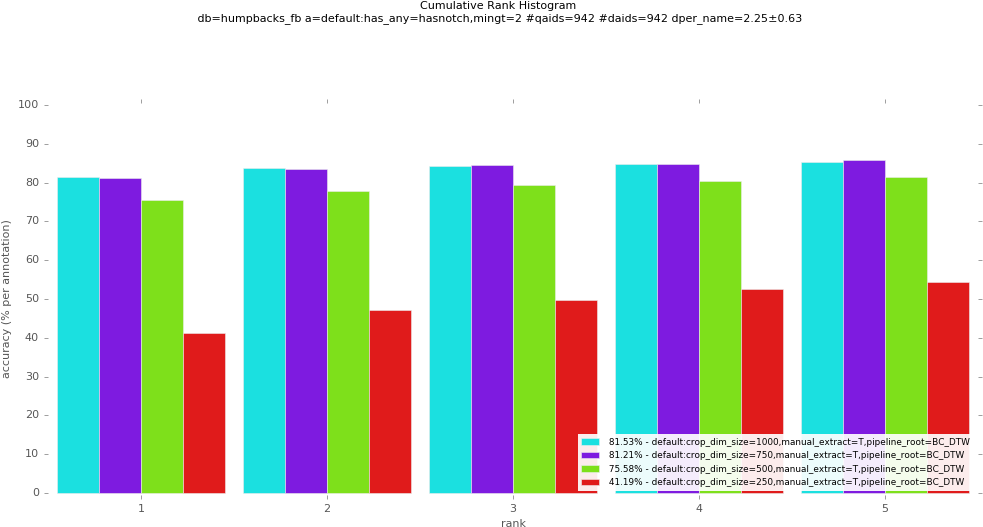
\includegraphics[width=1\textwidth]{../images/results/vary_crop_size.png}
\caption{\textbf{Varying $w$}. Note that we use the manually annotated points in this analysis to control for any issues with keypoint extraction.}
\label{fig:vary_crop_size}
\end{figure*}


\subsubsection{Trailing Edge Scorer Architecture}

The various trailing edge scorer architectures and their results on the task they were trained for is detailed in the previous chapter (see Table \ref{tab:te_score_full_analysis}).
In Figure \ref{fig:vary_te_scorer} we present the actual matching accuracies that each one produced with the mixing parameter $\beta = 0.5$.
We can see that the detailed and higher quality trailing edges produced by the Residual network give a decent performance boost over the other networks, however this performance boost appears to consist mostly of insignificant changes in query to ground truth distance.

\begin{figure*}[t]%
\centering
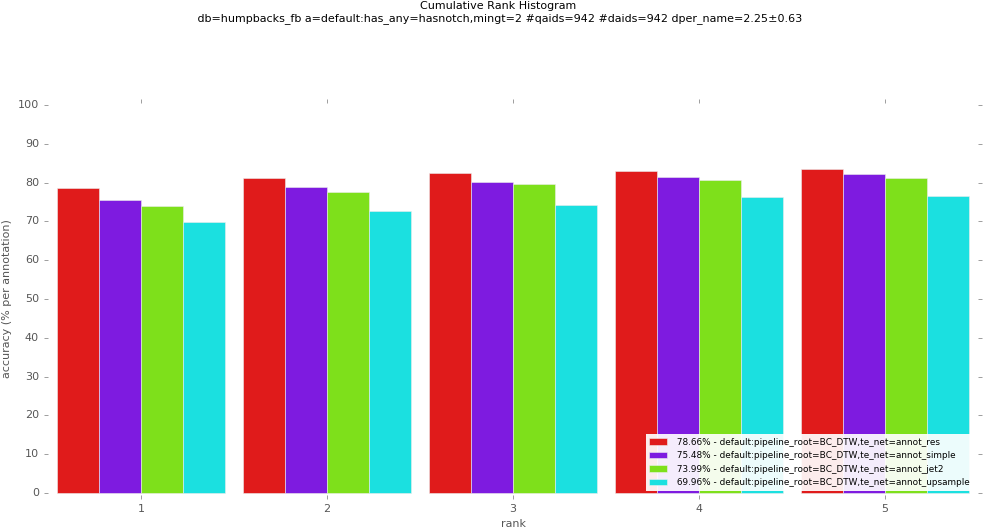
\includegraphics[width=1\textwidth]{../images/results/vary_te_scorer.png}
\caption{\textbf{Trailing Edge Scorer Architectures}. The highest performing trailing edge scorer (Residual) is shown in red, followed by Simple, Jet, and Upsample (in descending order of accuracy).}
\label{fig:vary_te_scorer}
\end{figure*}

A better evaluation of each trailing edge scoring architecture is given in Figure \ref{fig:vary_te_scorer_maxweight} where we only use the trailing edge scorer outputs to extract the trailing edge (i.e.\ $\beta = 1.0$).
Unsurprisingly, since the Upsample network gives blocky trailing edges (see Figure \ref{fig:example_te_scores_all}), it performs very poorly.
However in this case, no other network performs poorly, showing that the biggest issue is the low quality trailing edges that are extracted, not so much the lack of breaks in trailing edges.

\begin{figure*}[t]%
\centering
\includegraphics[width=1\textwidth]{../images/results/vary_te_scorer_maxweight.png}
\caption{\textbf{Trailing Edge Scorer Architectures at $\beta = 1$}. Upsample (cyan) performs significantly worse than the other networks, which all perform comparably.}
\label{fig:vary_te_scorer_maxweight}
\end{figure*}

One caveat with using the Residual network is that, with 64 layers, it consumes a lot of GPU memory when running.
This is currently an implementation issue, and the machine that carried out these experiments can handle it.
However, given that each network performs comparably, the Simple network is a good choice in general.

\subsubsection{Using a Trailing Edge Scorer}

In Figure \ref{fig:vary_te_weight}, we can see that simply a pixel-wise average of $N_y$ and $(1-T_y)$ (i.e. $\beta = 0.5$) produces the best results for the Residual network, though the differences are largely insignificant.
However, not using the trailing edge scorer (i.e.\ $\beta = 0$) performs significantly worse than using one at all (even with a low weight).
We show an example case where trailing edge scoring helps in Figure \ref{fig:dis_te_use}.

\begin{figure*}[t]%
\centering
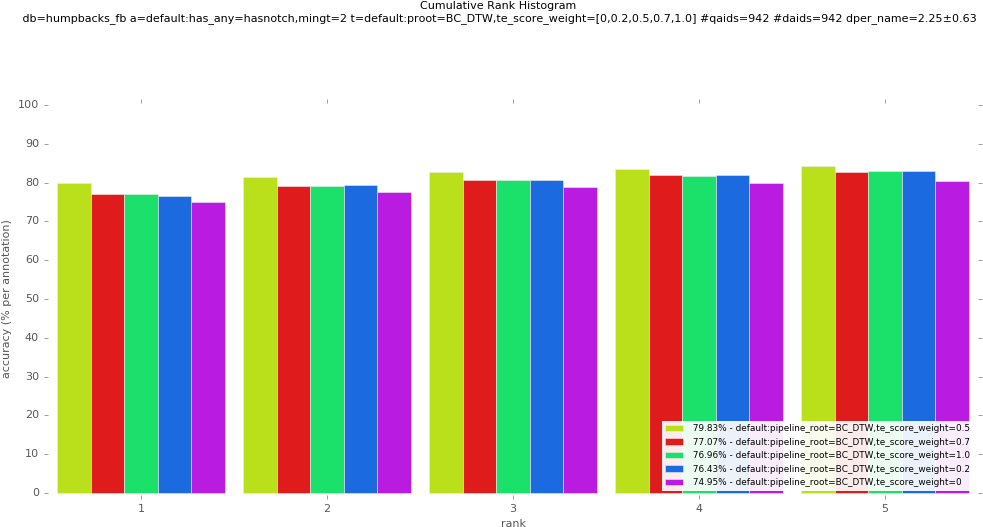
\includegraphics[width=1\textwidth]{../images/results/vary_te_weight.png}
\caption{\textbf{Varying $\beta$}. Setting $\beta = 0.5$ (yellow) provides only marginally better results over any other non-zero value of $\beta$, but is significantly better than $\beta = 0$ (purple).}
\label{fig:vary_te_weight}
\end{figure*}


\subsubsection{Number of neighbors in the extraction}

The number of neighbors $n$ effectively limits the slope of the trailing edge.
We limit it to an odd number for convenience.
On the one hand, a lower $n$ can cause the trailing edge to be limited in vertical breadth, but does prevent it from going way off course.
Despite this, with trailing edge scoring in place, it might be beneficial to increase $n$ so as to avoid parts of the trailing edge that continually ``max out'' the number of neighbors.

\begin{figure*}[t]%
\centering
\subfloat[][$\beta = 0.5$]{
	\includegraphics[width=0.5\textwidth]{../images/results/aid207_te_kp_overlay.png}
}
\subfloat[][$\beta = 0$]{
	\includegraphics[width=0.5\textwidth]{../images/results/aid207_te_kp_overlayno_tescorer.png}
}
\newline
\subfloat[][$T_p$]{
	\includegraphics[width=0.5\textwidth]{../images/results/aid207_tescorer_annot_res.png}
}
\subfloat[][$I_y$]{
	\includegraphics[width=0.5\textwidth]{../images/results/aid207_grad.png}
}
\caption{\textbf{Example Use of Trailing Edge Scorer}. In (a), we have the trailing edge extracted with the Residual scorer. Compare to (b), which did not use any scorer at all, resulting in a match failure.}
\label{fig:dis_te_use}
\end{figure*}

Ultimately, we can see in Figure \ref{fig:vary_neighbors} that limiting the number of neighbors to the immediate neighborhood (i.e. $n = 3$) produces a significant boost over a larger neighborhood.
We hypothesize that the trailing edges extracted with $n = 3$ are necessarily less detailed, and as a result can be more invariant to slight changes in pose of the fluke.
%Figure \ref{fig:dis_neighbors} presents an example case where, when using a higher number of neighbors, the notch is captured more faithfully --- but this introduces differences between the query and ground truth trailing edges that impede matching.
While this effect is only present in a small number of cases, the difference in accuracy here is significant, with 78\% of the improvements resulting in a score difference over $\epsilon$.

\begin{figure*}[t]%
\centering
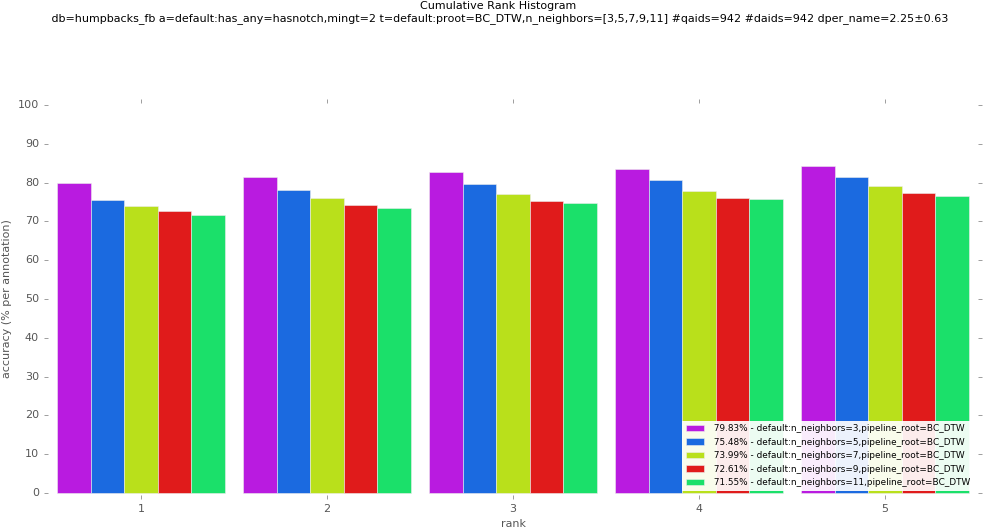
\includegraphics[width=1\textwidth]{../images/results/vary_neighbors.png}
\caption{\textbf{Varying $n$}. This shows that the optimal neighborhood constraint is $n = 3$ (purple), despite qualitatively producing worse-looking trailing edges. After $n = 5$ (blue), the trailing edges can become very noisy affecting match accuracy.}
\label{fig:vary_neighbors}
\end{figure*}

\subsubsection{Using the notch}

Initially, we believed that using the notch as a control point (i.e.\ forcing the trailing edge to go through the notch) would give better trailing edges, and therefore an increase in accuracy.
As it turns out, this is not the case --- using the notch as a control point gives somewhat worse accuracy.
Surprisingly, this decrease in matching accuracy holds for both manually annotated and automatically extracted keypoints.
However, most of these discrepancies did not result in a score difference above $\epsilon$.
This could be because of the small difference in trailing edge between those with the notch as a part of the trailing edge and those without, which leads to matching failure but not a large difference in score.

%\begin{figure*}[t]%
%\centering
%\includegraphics[width=1\textwidth]{../images/results/vary_ignore_notch.png}
%\caption{\textbf{Using the notch as a control point}. Ignoring the notch point (cyan) gives better accuracy than using the notch point (red).}
%\label{fig:vary_notch}
%\end{figure*}

\subsection{Curvature Scales}

Computing the curvature is one of the least parameterized parts of the process, however figuring out what the optimal scales to extract are and how many to compute is non-trivial.
Instead of exhaustively exploring these options, we can use some heuristics to determine which curvature scales to explore.
Each scale as measures the curvature of some percentage of the trailing edge around each point on the trailing edge.
Intuitively, we want to capture the curvature at a scale that provides the most variation between trailing edges.
Therefore, in order to determine which scales to measure, we look at how much the actual curvature changes between successive scales, as well as the average variance in curvature among trailing edges at each scale. 

\begin{figure*}[t]%
\centering
\subfloat[][]{
	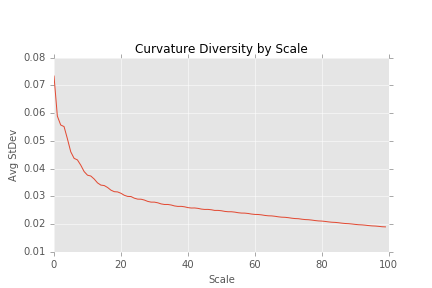
\includegraphics[width=0.5\textwidth]{../images/results/curvature_diversity_fb.png} 
	\label{fig:curvature_diversity:a}
}
\subfloat[][]{
	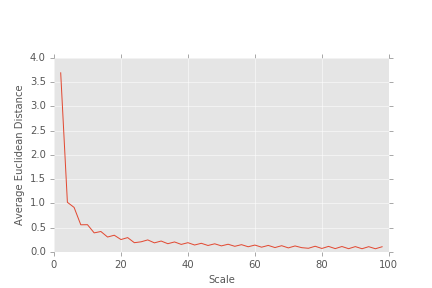
\includegraphics[width=0.5\textwidth]{../images/results/interscale_diff_fb.png} 
	\label{fig:curvature_diversity:b}
}%
\caption{\textbf{Curvature Diversity}. Left panel (a) shows the average standard deviation of the (fixed length) curvature at different scales. Right panel (b) shows the average Euclidean distance between curvatures measured at successive scales.}
\label{fig:curvature_diversity}
\end{figure*}

We find that (as shown in the Figure \ref{fig:curvature_diversity:b}) as block curvature scale is increased, the diversity at any given point in the curvature goes down drastically (as expected). 
Therefore, we stick to the lower end of the scale, keeping the curvature scales measured below $10\%$.
We can also see in Figure \ref{fig:curvature_diversity:a} that successive curvature scales show bigger differences at lower scales than at higher scales, which reinforces using curvatures below $10\%$, but also encourages bigger jumps between scales to maximize diversity while minimizing computation time.
Based on the above, we evaluated scales that run from $1\%$ to $10\%$, with varying levels of resolution, and found little to no significant effect on matching accuracy compared to using the default set of scales.

%\begin{figure*}[t]%
%\centering
%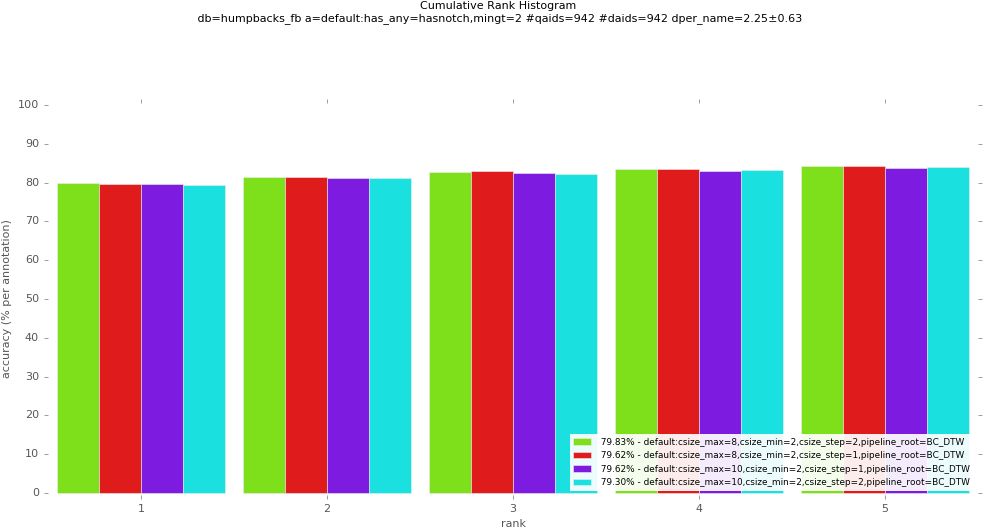
\includegraphics[width=1\textwidth]{../images/results/vary_curv_scales.png}
%\caption{\textbf{Varying Curvature Scales}. The scales evaluated here are parameterized with a start, end, and step size. We always start at 2\%, and vary the step size between 1 \& 2 and the end between 8\% \& 10\%.}
%\label{fig:vary_curv_scales}
%\end{figure*}

\subsection{Sakoe-Chiba bound}

%The main variants shown in this section are the different Sakoe-Chiba bound windows and the scale weighting term in the curvature distance function.

%\subsubsection{Weighting the different scales}

%There are many ways to produce the weights $s_w$ for curvatures, but intuitively there should be a monotonic relationship between curvature scale and importance.

%We could specify this relationship as a ratio $W$ of importance between successive pairs of curvatures (increasing in size).
%We parameterize that importance by giving each scale the weight $s_w = [W^i \forall i \in [0,|S|]$.
%In order to maintain this ratio without blowing up the distances, we also normalize so that $\sum s_w = 1$.

%\begin{figure*}[t]%
%\centering
%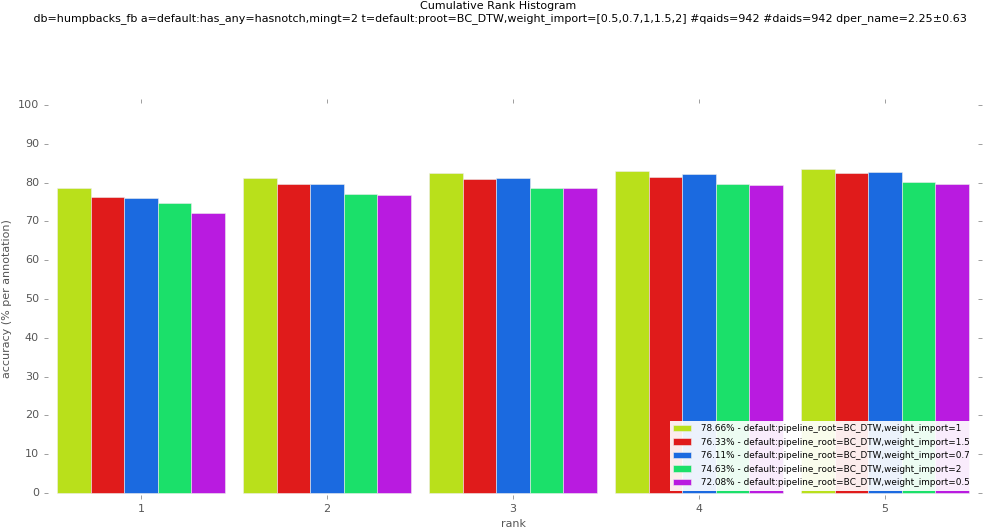
\includegraphics[width=1\textwidth]{../images/results/vary_weight_import.png}
%\caption{\textbf{Varying $s_w$}. The yellow bar shows $W = 1$, i.e.\ all curvatures weighted equally.}
%\label{fig:vary_weight_import}
%\end{figure*}



%Figure \ref{fig:vary_weight_import} shows that despite this effort, it appears that equally weighting each curvature scale provides the best performance.
%Interestingly weighting larger scales lower (i.e.\ $W < 1$, which we evaluate with $W = 0.5$ (purple bar) in Figure \ref{fig:vary_weight_import}) provides worse performance.

\begin{figure*}[t]%
\centering
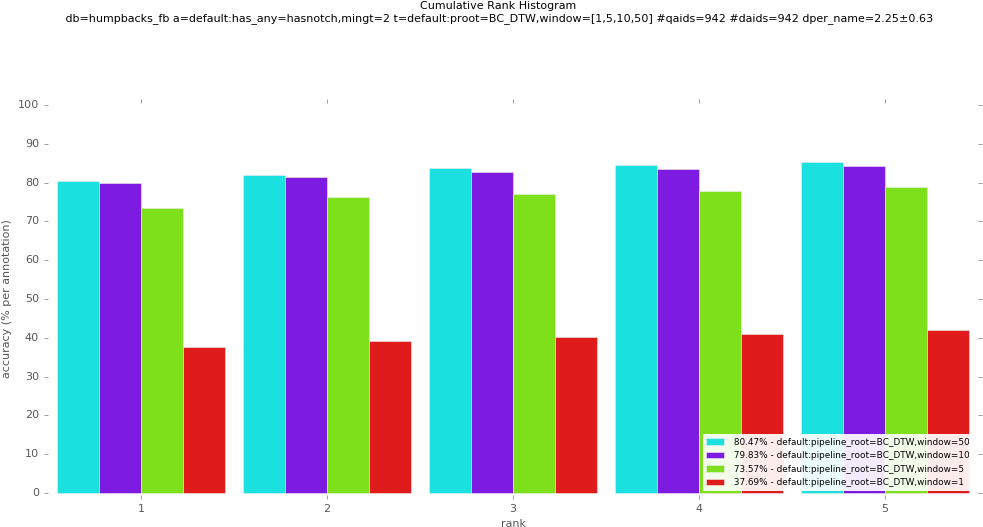
\includegraphics[width=1\textwidth]{../images/results/vary_window.png}
\caption{\textbf{Varying Sakoe-Chiba Bound}. We achieve good results with the Sakoe-Chiba bound set to $10\%$ (yellow), although we can get slightly better results with it set to $50\%$ (green) at the expense of computation time.}
\label{fig:vary_window}
\end{figure*}



In Figure \ref{fig:vary_window}, we can see that if we decrease the window (i.e. the Sakoe-Chiba bound) size, at around 10\% of the query trailing edge length we maintain only slightly worse accuracy compared to the full window (i.e. 100\%), but below this accuracy is severely affected.
We find that overall there is a $4\times$ slow-down in wall-clock time on our testing machine\footnote{The CPU used is a 6-core Intel i7 clocked at 3.5GHz} when going from a window size of 10\% to one of 100\%. 
Thus, we use this value for the window size so as to minimize computation time while maintaining the total accuracy.
Additionally, while it's possible for gross mismatches to occur from there being no window boundary, we can see from Figure \ref{fig:vary_window} that this does not pose a problem.

%\subsubsection{Aggregating over multiple trailing edges per identity}

%Determining the identity of a given query image given distances to other images in the database is not entirely simple when there are multiple database images for a given individual.
%Essentially we need to transform these distances from query image to database image into distances from query to known individual.
%To do so we evaluate two options given a group of distances for an individual --- either the average distance or the minimum distance.

%We find that the average decision does slightly better, as shown in Figure \ref{fig:vary_decision}.

%This is unsurprising given that most of the individuals in the dataset only have two images associated, meaning that the average is equivalent to the minimum.
%That said, the minimal distance criterion is effectively the single-feature case of LNBNN used in Hotspotter \cite{crall_hotspotter_2013} and the work of Hughes et al.\ \cite{hughes2015automated}. % Maybe: prove this?

%\begin{figure*}[t]%
%\centering
%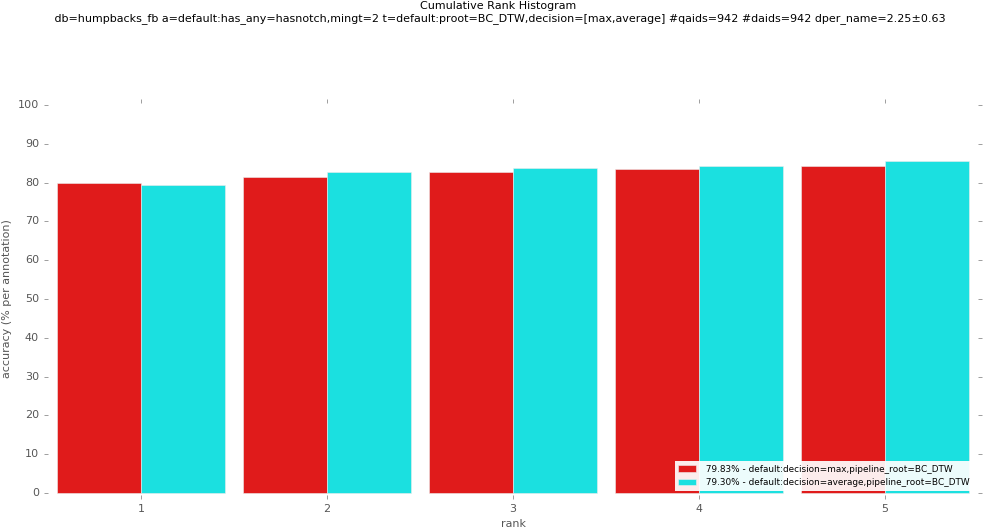
\includegraphics[width=1\textwidth]{../images/results/vary_decision.png}
%\caption{\textbf{Varying Decision Criterion}}
%\label{fig:vary_decision}
%\end{figure*}

\section{In Combination with Hotspotter}

\begin{figure*}[t]%
\centering
\subfloat[][]{
	\includegraphics[width=0.5\textwidth]{../images/results/aid493_te_kp_overlay.png}
}
\subfloat[][]{
	\includegraphics[width=0.5\textwidth]{../images/results/aid147_te_kp_overlay.png}
}
\newline
\subfloat[][]{
	\includegraphics[width=0.5\textwidth]{../images/results/aid494_te_kp_overlay.png}
}
\subfloat[][]{
	\includegraphics[width=0.5\textwidth]{../images/results/aid148_te_kp_overlay.png}
}
\caption{\textbf{Example Disagreements Between Hotspotter and our method}. On the left side, (a) was matched correctly to (c) by our method, whereas Hotspotter could not find any matches for (a). On the right hand side however, Hotspotter was able to match two flukes with a large variance in pose and lighting, while our method did not rank (d) in the top 5 matches for (b).}
\label{fig:dis_proot}
\end{figure*}



Comparatively, our method gets a slightly better top-1 accuracy than Hotspotter (see Figure \ref{fig:vary_proot})
However, our method targets a specific part of the fluke whereas Hotspotter recognizes general patterns, and thus can make use of the internal texture of the fluke.
Therefore, by combining our method with Hotspotter --- if we were able to automatically pick out which algorithm was right for a given ranking --- we would expect to see a significant increase in accuracy.
We find that in this ideal scenario, we can achieve a 93\% top-1 accuracy on the Flukebook dataset.
However, automatically deciding which algorithm to use for matching is non-trivial, and we are still exploring it.

See Figure \ref{fig:dis_proot} for an example where Hotspotter correctly finds a match where our method fails, and vice-versa.

\subsection{Characterization of when to use which method}

From an intuitive standpoint, it appears that Hotspotter cannot find effective keypoints from trailing edges, which hampers its ability to handle flukes which do not have an apparent pattern.

We hypothesize that this is because the trailing edge --- while a distinctive feature --- inevitably shares a region with an oceanic background.
Since this oceanic background changes from image to image, it cannot verify salient keypoints as matches.
As a result, flukes which have little to no internal texture are nearly impossible for Hotspotter to match.

\begin{figure*}[t]%
\centering
\includegraphics[width=1\textwidth]{../images/results/vary_proot.png}
\caption{\textbf{Comparison between Hotspotter and our method}. Hotspotter's accuracy (cyan) is slightly worse than our method's (red), however we find that they are fairly complementary. Note that Hotspotter's accuracy does not increase much with allowed matching rank.}
\label{fig:vary_proot}
\end{figure*}



On the other hand, when the trailing edge is unclear or significantly distorted in the image, our method struggles to find an appropriate match.
In these cases, Hotspotter can provide a good match, although if the fluke is additionally untextured we have an issue.
We were unable to find a single heuristic that correlates with our method failing to find a match.
Particularly we find that smoothness of the trailing edge, characterized by the standard deviation of the trailing edge slope, does not correlate to match failure.
This implies that smooth trailing edges are about as easy to match for our method as rough, distinctive trailing edges.
However, since the dataset we use consists primarily of individuals with only two images, failures can occur for a variety of reasons.


%%% Local Variables: 
%%% mode: latex
%%% TeX-master: t
%%% End: 
 % chapter 4
%%%%%%%%%%%%%%%%%%%%%%%%%%%%%%%%%%%%%%%%%%%%%%%%%%%%%%%%%%%%%%%%%%% 
%                                                                 %
%                            CHAPTER FIVE                          %
%                                                                 %
%%%%%%%%%%%%%%%%%%%%%%%%%%%%%%%%%%%%%%%%%%%%%%%%%%%%%%%%%%%%%%%%%%% 

\chapter{Discussion} \label{sec:discussion}

\section{Issues with the Proposed Method}

\begin{figure*}[t]%
\centering
\includegraphics[width=1\textwidth]{../images/results/bc_dtw_gtrank_hist.png}
\caption{\textbf{Histogram of Ground-Truth Ranks}. Note that the histogram ranges are uneven to better show the lower end of the range. In order to have all matches found within the top-$k$ matches we would have to set $k = 414$.}
\label{fig:gtrank_hist}
\end{figure*}

The primary issue that we encountered is that whether or not a given pair of trailing edges belongs to the same individual based solely on the distance between them is difficult (see Figure \ref{fig:score_sep}).
This hinders finding a threshold distance such that below it we can consider a pair of trailing edges to match (i.e.\ a verification task).
A side effect of this is that small changes in the trailing edge can lead to matching failures, and in the worst case ``push down'' the correct match's rank significantly.
This affects the usability of our method, as ideally a human operator verifying a match would only have to look at the top-$k$ flukes for some small value $k$.
However, we find that in many failure cases the correct match is far down the list, and there is no reasonable value $k$ (i.e.\ that a human operator would want to find a match in) that all matches are within (see Figure \ref{fig:gtrank_hist}). 

While this handling of failure cases is suboptimal, Figure \ref{fig:score_diff1st2nd} shows that by thresholding the difference in scores between the first and second ranked flukes for a given query, we can determine with high confidence whether or not a given query is matched correctly.
However, we cannot easily ascertain a failure case from this, as there are many success cases that overlap with score differences that characterize failure cases.


There are several other issues with our method, primarily having to do with the stability and generalization capability of the convolutional networks used for fluke keypoint predictions and trailing edge scores.
For the former network, ideally the keypoints could be predicted without needing our assumption on fluke position and orientation, although it is clear to us that this does not happen.
We believe that this is primarily due to the lack of training data that defies these assumptions, although it is also possible that it is beyond the capacity of the models we trained.
That said, having the fluke horizontally oriented and flat to the camera does not only help the keypoint extraction, but also avoids an obscured trailing edge due to out-of-plane rotations (as seen in Figures \ref{fig:example_kp_failure} and \ref{fig:unclear_te}) --- so these assumptions that we make help get a good trailing edge.
However, imposing this requirement complicates and restricts the actual photography of these flukes by requiring the photographer to be in a very specific position with respect to the subject fluke.


We noted that for the trailing edge extractor, it would often use the gradient information to define a trailing edge rather than some deeper semantic image properties (see Figure \ref{fig:example_te_res_failure}).
Part of the reason for this is similar in nature to the problem for training the fluke keypoint network, i.e.\ that a large majority of the dataset represent ``easy'' cases (where the gradient signal correlates with the trailing edge), making it hard to train the network to handle hard cases.
We did use data augmentation to help rectify this bias, but it was not completely effective.
It is possible that more sophisticated data augmentation could help, but primarily we think that spending more time annotating and creating a trailing edge scoring dataset would be ideal.

\section{Future work}

\begin{figure*}[t]%
\centering
\subfloat[][] {
	\includegraphics[width=0.5\textwidth]{../images/results/score_diff_fail_hist.png}
}
\subfloat[][] {
	\includegraphics[width=0.5\textwidth]{../images/results/score_diff_succ_hist.png}
}
\caption{\textbf{Histogram of Score Differences between 1st and 2nd Rank}. Note that the histogram ranges are uneven to better show the higher	end of the range.}
\label{fig:score_diff1st2nd}
\end{figure*}



There is a lot of work that can be done based on this method.
The immediate focus is to achieve the theoretical 93\% accuracy by accurately choosing to use either Hotspotter or our method for any given query and resultant ranking over possible matches.
This would result in a more general method that could be robust to obscured trailing edges and some out-of-plane rotations, while also handling untextured flukes.

One part of this identification pipeline that we mostly ignored is a detection and orientation step.
While orientation is not necessarily important for the curvature measure (as it is rotation invariant), it is important for the trailing edge extraction.
Additionally, being able to detect and crop the fluke automatically from an image would give a much more robust and flexible system.
We did not explore this as most of the images in the Flukebook dataset came pre-cropped around the fluke, as well as rotated such that the major axis of the trailing edge was horizontal.
These conditions both obviate the need for such a system and make it difficult to train a detection and orientation model.

Extracting the trailing edge is currently done with an unsophisticated and restricted algorithm, which can be improved. 
There are several ways to improve this algorithm, but the main drawbacks are its lack of rotation invariance and the inability to easily determine the second or third best trailing edge.
On top of that, the trailing edge scoring networks could be better evaluated with more annotated trailing edges, the creation of which is non-trivial.

There is a lot to be done with the matching algorithm itself, namely in ensuring that it is more tolerant to insignificant deformations in the trailing edge.
One major paradigm that we do not explore in this work is that of extracting and matching multiple features per trailing edge, much in the same way that Hotspotter and Hughes et al.\ \cite{hughes2015automated} operate.

\section{Conclusion}

In this thesis we have presented a novel, fully-automated method for photo-identifying humpback flukes that achieves a high top-1 ranking accuracy on a relatively large dataset.
This method extracts fine grained trailing edge contours from images of flukes and identifies individuals based on sequence properties of the contour curvature.

%%% Local Variables: 
%%% mode: latex
%%% TeX-master: t
%%% End: 
 % chapter 5
%%%%%%%%%%%%%%%%%%%%%%%%%%%%%%%%%%%%%%%%%%%%%%%%%%%%%%%%%%%%%%%%%%% 
%                                                                 %
%                           BIBLIOGRAPHY                          %
%                                                                 %
%%%%%%%%%%%%%%%%%%%%%%%%%%%%%%%%%%%%%%%%%%%%%%%%%%%%%%%%%%%%%%%%%%% 
 
%This method produces a numbered bibliography where the numbers
%correspond to the \cite commands in the text. See the LaTeX manual.
%
\let\cleardoublepage\clearpage

\begin{singlespace}

\bibliographystyle{abbrv}
\renewcommand{\bibname}{\specialhead{REFERENCES}}
\bibliography{references}

\end{singlespace}

% Note that, if you wish, you can use BibTeX to create your bibliography
% from a database. See section 5.6.2 of Memo RPI.110 for information. 
%%% Local Variables: 
%%% mode: latex
%%% TeX-master: t
%%% End: 
 % bibliography
%%%%%%%%%%%%%%%%%%%%%%%%%%%%%%%%%%%%%%%%%%%%%%%%%%%%%%%%%%%%%%%%%%%
%                                                                 %
%                            APPENDICES                           %
%                                                                 %
%%%%%%%%%%%%%%%%%%%%%%%%%%%%%%%%%%%%%%%%%%%%%%%%%%%%%%%%%%%%%%%%%%%
 
\appendix    % This command is used only once!
%\addcontentsline{toc}{chapter}{APPENDICES}             %toc entry  or:
\addtocontents{toc}{\parindent0pt\vskip12pt APPENDIX} %toc entry, no page #


\chapter*{APPENDIX} \label{sec:appendix}


 % appendix
 
\end{document}
